\documentclass[12pt,a4paper]{article}

\usepackage[top=1in, bottom=1in, left=1in, right=1in]{geometry}
\usepackage{graphicx}
\usepackage{amsmath}
\usepackage{array}
\usepackage{hyperref}

\hypersetup{
    colorlinks=true,
    linkcolor=black,
    urlcolor=black,
    citecolor=black
}

\graphicspath{{images/}}
\setlength{\emergencystretch}{2em}

\begin{document}

\hypersetup{pageanchor=false}
\begin{titlepage}
\thispagestyle{empty}
\begin{center}
    {\large Erasmus Mundus Joint Master's Degree in Artificial Intelligence}\\[0.15cm]
    {\large for Image Processing and Computer Vision}\\[0.25cm]
    {\large Universidad Aut\'onoma de Madrid}

    \vspace{3.0cm}

    \rule{0.82\textwidth}{0.6pt}\\[0.65cm]
    {\LARGE\bfseries 3D Vision for Multiple and Moving Cameras}\\[0.35cm]
    {\Large Lab Evaluation Report}\\[0.65cm]
    \rule{0.82\textwidth}{0.6pt}

    \vspace{2.3cm}

    {\Large Gourab Roy}
\end{center}
\end{titlepage}
\hypersetup{pageanchor=true}
\pagenumbering{arabic}

\tableofcontents
\clearpage

% ============================================================
\section{Obtention of the Intrinsic Parameters of a Camera}
% ============================================================

This section describes the camera calibration procedure carried out using
Zhang's homography-based calibration method. Two independent calibration patterns were used:
(1)~the provided digital checkerboard displayed on a laptop screen, and
(2)~a custom physical pattern consisting of floor-tile grid intersections.  The
resulting intrinsic matrices $\mathbf{A}$ and $\mathbf{A}'$ are analysed
quantitatively and compared below.

% ------------------------------------------------------------
\subsection{Screen-Checkerboard Calibration}
\label{sec:screen_calib}
% ------------------------------------------------------------

\subsubsection*{Acquisition setup}

The provided $1080\,\mathrm{px}$ checkerboard image was opened in full-screen
mode on a laptop display so that it covered the entire screen area, simulating a
physical checkerboard.  The camera was hand-held and moved to seven distinct
viewpoints, ensuring substantial variation in tilt, rotation, and distance.
The captured images have a resolution of $1530 \times 2040\,\mathrm{px}$.
All seven images were successfully used for calibration (no image was rejected by
the corner detector).

Key acquisition parameters are summarised in Table~\ref{tab:screen_setup}.

\begin{table}[htbp]
\centering
\caption{Screen-checkerboard acquisition parameters.}
\label{tab:screen_setup}
\begin{tabular}{ll}
\hline
Parameter & Value \\
\hline
Image resolution & $1530 \times 2040\,\mathrm{px}$ \\
Valid calibration images & 7 \\
Screen checkerboard width & $182.6000\,\mathrm{mm}$ \\
Detected board size & $[8 \times 8]$ inner corners \\
Square size & $22.825000\,\mathrm{mm}$ \\
\hline
\end{tabular}
\end{table}

Figure~\ref{fig:montage_screen} shows the montage of all seven calibration images.

\begin{figure}[htbp]
    \centering
    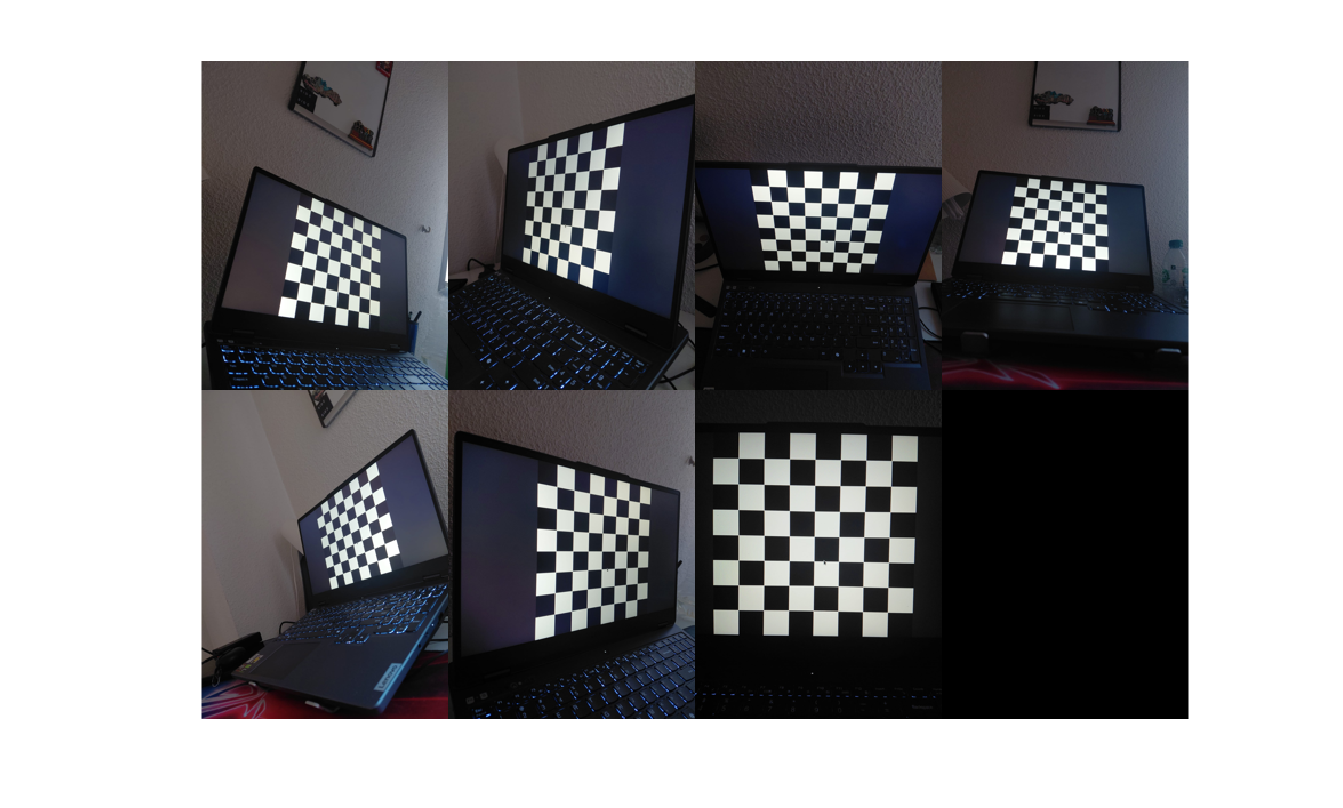
\includegraphics[width=\textwidth]{section_1/montage_screen.png}
    \caption{Montage of the seven screen-checkerboard calibration images used to
             estimate $\mathbf{A}$.}
    \label{fig:montage_screen}
\end{figure}

\subsubsection*{Intrinsic matrix}

The Zhang calibration procedure produced the following intrinsic matrix:

\begin{equation}
\mathbf{A} =
\begin{bmatrix}
1530.2905 & -13.9038 & 765.0597 \\
0         & 1526.9686 & 1085.4281 \\
0         & 0          & 1
\end{bmatrix}
\label{eq:A_screen}
\end{equation}

\noindent where $\alpha = A_{11}$ and $\beta = A_{22}$ are the focal lengths
in pixels along the $u$- and $v$-axes respectively, $\gamma = A_{12}$ is the
skew coefficient, and $(u_0, v_0) = (A_{13}, A_{23})$ is the principal point.

Table~\ref{tab:screen_metrics} lists the full set of derived calibration metrics.

\begin{table}[htbp]
\centering
\caption{Quantitative metrics derived from the screen-checkerboard intrinsic matrix
         $\mathbf{A}$.}
\label{tab:screen_metrics}
\begin{tabular}{lr}
\hline
Metric & {Value} \\
\hline
$\alpha$ (focal length, $u$-axis) [px]     & 1530.290478 \\
$\beta$ (focal length, $v$-axis) [px]      & 1526.968553 \\
$\gamma$ (skew) [px]                       & -13.903781  \\
$u_0$ (principal point, $u$) [px]          & 765.059672  \\
$v_0$ (principal point, $v$) [px]          & 1085.428138 \\
Aspect ratio $\alpha/\beta$                & 1.002176    \\
Aspect-ratio deviation from 1 [\%]        & 0.217550    \\
Principal-point offset from image centre [px] & 65.428165 \\
Principal-point offset [\% of half-diagonal]  & 5.131621  \\
Orthogonality deviation from $90^\circ$ [deg] & 0.520559  \\
Mean reprojection error [px]               & 9.763672    \\
\hline
\end{tabular}
\end{table}

\subsubsection*{Quantitative analysis}

\paragraph{Pixel squareness.}
The aspect ratio $\alpha/\beta = 1.002176$ deviates from unity by only
$0.2176\%$, indicating that the camera pixels are very nearly square.
This result is consistent with modern CMOS sensors whose pixel pitch is
equal in both directions.

\paragraph{Principal point location.}
The horizontal offset of the principal point from the image centre is
$\Delta u = u_0 - W/2 = 765.0597 - 765 = 0.0597\,\mathrm{px}$,
which is negligible.  The vertical offset is
$\Delta v = v_0 - H/2 = 1085.4281 - 1020 = 65.4281\,\mathrm{px}$,
placing the principal point slightly below the geometric centre.
The Euclidean offset from the centre is $65.43\,\mathrm{px}$,
corresponding to $5.13\%$ of the half-diagonal.  This offset is small but
non-zero, as expected for a consumer lens that is not perfectly centred.

\paragraph{Axis orthogonality.}
The skew parameter $\gamma = -13.904\,\mathrm{px}$ is small relative to
the focal lengths ($|\gamma|/\alpha < 1\%$).  The derived orthogonality
deviation is $0.521^\circ$, confirming that the image axes are very
nearly perpendicular.

\paragraph{Reprojection quality.}
Figure~\ref{fig:reproj_screen} shows the detected corner positions (green
circles) overlaid with the reprojected corner positions (red crosses) for
the first calibration image.

\begin{figure}[htbp]
    \centering
    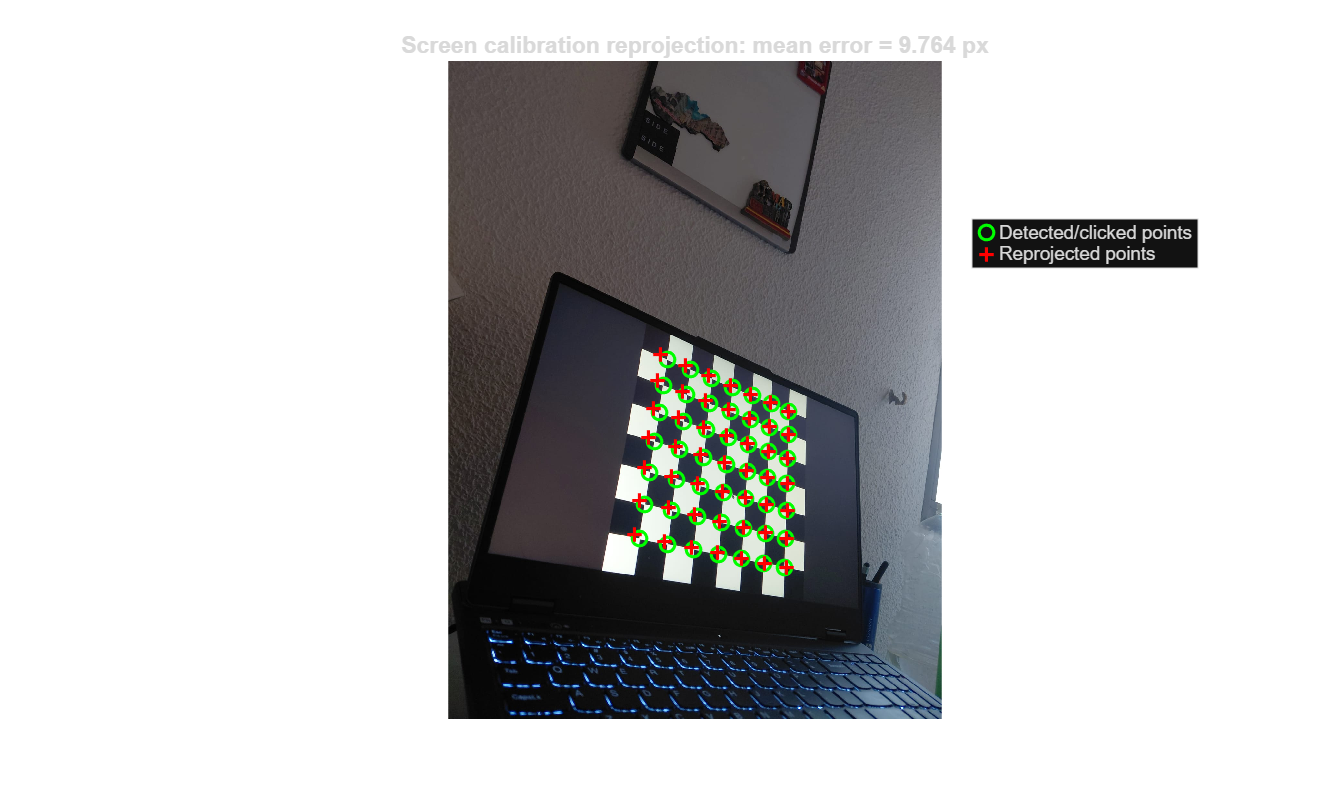
\includegraphics[width=0.75\textwidth]{section_1/reprojection_screen.png}
    \caption{Reprojection check for screen-checkerboard calibration:
             detected corners (green circles) vs.\ reprojected corners
             (red crosses) on image~1.  Mean reprojection error: $9.764\,\mathrm{px}$.}
    \label{fig:reproj_screen}
\end{figure}

The mean reprojection error is $9.764\,\mathrm{px}$.  Although this value
is higher than what a standard sub-pixel accurate detector would yield for
a printed calibration target, it is attributable to the reflective
properties of the screen surface (glare, Moir\'{e} patterns at certain
angles) and to moderate hand-motion blur in some views.  The consistent
spread of detected and reprojected points across the board nevertheless
confirms that $\mathbf{A}$ is geometrically sound.

% ------------------------------------------------------------
\subsection{Custom Physical Pattern Calibration}
\label{sec:custom_calib}
% ------------------------------------------------------------

\subsubsection*{Pattern selection rationale}

A floor-tile planar $3 \times 3$ grid was chosen as the custom calibration
pattern.  The tiles are made of ceramic with sharp, contrasting grout lines
whose intersections form a regular grid.  The following considerations
motivated this choice:
\begin{itemize}
    \item \textbf{Planarity:} the floor surface is flat to within fractions
          of a millimetre, satisfying the planarity assumption of Zhang's method.
    \item \textbf{Physical measurability:} the tile dimensions were measured
          with a tape measure, yielding a tile side of $330\,\mathrm{mm}$,
          which defines the world coordinate system directly.
    \item \textbf{Environmental availability:} no special equipment was needed;
          the pattern was readily available in the capture environment.
    \item \textbf{Visible intersections:} the grout-line intersections are
          visually unambiguous and can be clicked precisely in each image.
\end{itemize}

Because the corner locations cannot be detected automatically (unlike a
printed checkerboard), the nine grid intersections were marked manually
in every image using an interactive point-selection tool.  The clicked
coordinates were saved in \path{results/section_1/custom_clicked_points.mat}
for reproducibility.

\subsubsection*{Acquisition setup}

Seven images of the floor-tile pattern were captured with the same camera
used in Section~\ref{sec:screen_calib}, keeping all internal settings fixed.
The images have the same resolution of $1530 \times 2040\,\mathrm{px}$.
In each image, the nine grid intersections were clicked row by row, left to
right, top to bottom.

Key acquisition parameters are summarised in Table~\ref{tab:custom_setup}.

\begin{table}[htbp]
\centering
\caption{Custom floor-tile pattern acquisition parameters.}
\label{tab:custom_setup}
\begin{tabular}{ll}
\hline
Parameter & Value \\
\hline
Pattern & Floor-tile planar $3\times3$ grid \\
Image resolution & $1530 \times 2040\,\mathrm{px}$ \\
Valid calibration images & 7 \\
Tile size & $330.0000\,\mathrm{mm}$ \\
Measured point layout & $3 \times 3$ grid, 9 points \\
Point selection & Manual (interactive click) \\
\hline
\end{tabular}
\end{table}

Figure~\ref{fig:montage_custom} shows the montage of the seven custom-pattern
calibration images.

\begin{figure}[htbp]
    \centering
    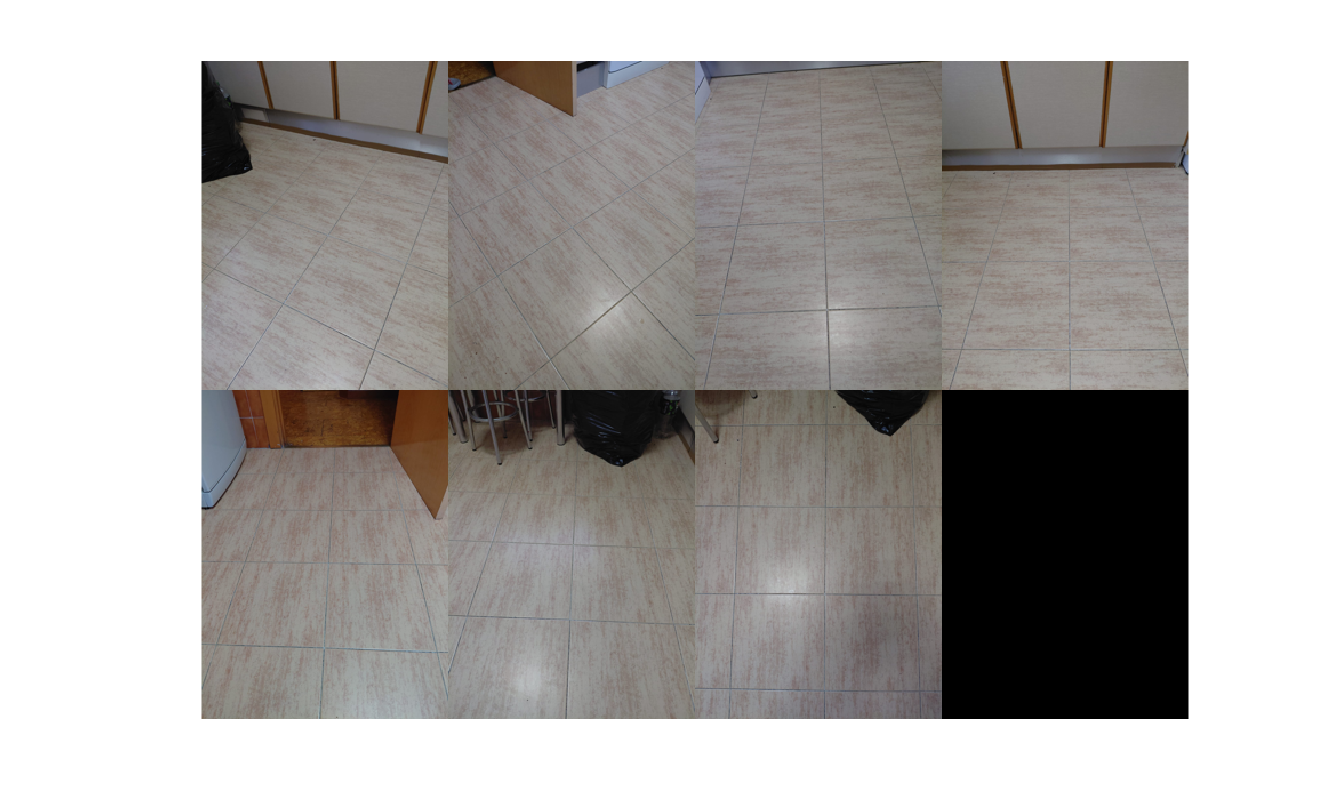
\includegraphics[width=\textwidth]{section_1/montage_custom.png}
    \caption{Montage of the seven floor-tile custom-pattern calibration images
             used to estimate $\mathbf{A}'$.}
    \label{fig:montage_custom}
\end{figure}

\subsubsection*{Intrinsic matrix}

Applying the same Zhang calibration procedure to the nine manually selected
points per image yields:

\begin{equation}
\mathbf{A}' =
\begin{bmatrix}
1784.2663 & 21.8624  & 823.0723 \\
0         & 1729.8189 & 779.8572 \\
0         & 0          & 1
\end{bmatrix}
\label{eq:A_custom}
\end{equation}

Table~\ref{tab:custom_metrics} lists the full set of derived metrics.

\begin{table}[htbp]
\centering
\caption{Quantitative metrics derived from the custom floor-tile intrinsic
         matrix $\mathbf{A}'$.}
\label{tab:custom_metrics}
\begin{tabular}{lr}
\hline
Metric & {Value} \\
\hline
$\alpha$ (focal length, $u$-axis) [px]     & 1784.266316 \\
$\beta$ (focal length, $v$-axis) [px]      & 1729.818897 \\
$\gamma$ (skew) [px]                       & 21.862362   \\
$u_0$ (principal point, $u$) [px]          & 823.072343  \\
$v_0$ (principal point, $v$) [px]          & 779.857214  \\
Aspect ratio $\alpha/\beta$                & 1.031476    \\
Aspect-ratio deviation from 1 [\%]        & 3.147579    \\
Principal-point offset from image centre [px] & 247.064677 \\
Principal-point offset [\% of half-diagonal]  & 19.377622  \\
Orthogonality deviation from $90^\circ$ [deg] & -0.702002  \\
Mean reprojection error [px]               & 15.359148   \\
\hline
\end{tabular}
\end{table}

\subsubsection*{Quantitative analysis}

\paragraph{Pixel squareness.}
The aspect ratio $\alpha/\beta = 1.031476$ deviates from unity by
$3.148\%$, noticeably more than the $0.218\%$ obtained from the screen
calibration.  Because the camera is the same physical device, the
discrepancy is attributed to calibration noise rather than genuine
pixel non-squareness: only nine manually clicked points per image are
available, providing far fewer geometric constraints than the
$8 \times 8 = 64$ automatically detected corners of the screen board.

\paragraph{Principal point location.}
The principal point $\mathbf{A}'$ is located at $(823.07,\,779.86)\,\mathrm{px}$,
with a horizontal offset $\Delta u = 58.07\,\mathrm{px}$ and a vertical
offset $\Delta v = -240.14\,\mathrm{px}$ (above the image centre).
The total Euclidean offset is $247.06\,\mathrm{px}$, corresponding to
$19.38\%$ of the half-diagonal, which is substantially larger than the
$5.13\%$ obtained from the screen calibration.  Such a large offset is a
strong indicator of under-constrained calibration from a sparse point set.

\paragraph{Axis orthogonality.}
The skew $\gamma = 21.862\,\mathrm{px}$ is larger in magnitude than the
screen value of $-13.904\,\mathrm{px}$, and the derived orthogonality
deviation is $-0.702^\circ$.  Although this remains close to orthogonal,
the increased skew is again consistent with the greater noise inherent in
manual point selection.

\paragraph{Reprojection quality.}
Figure~\ref{fig:reproj_custom} shows the reprojection check for the first
custom-pattern image.

\begin{figure}[htbp]
    \centering
    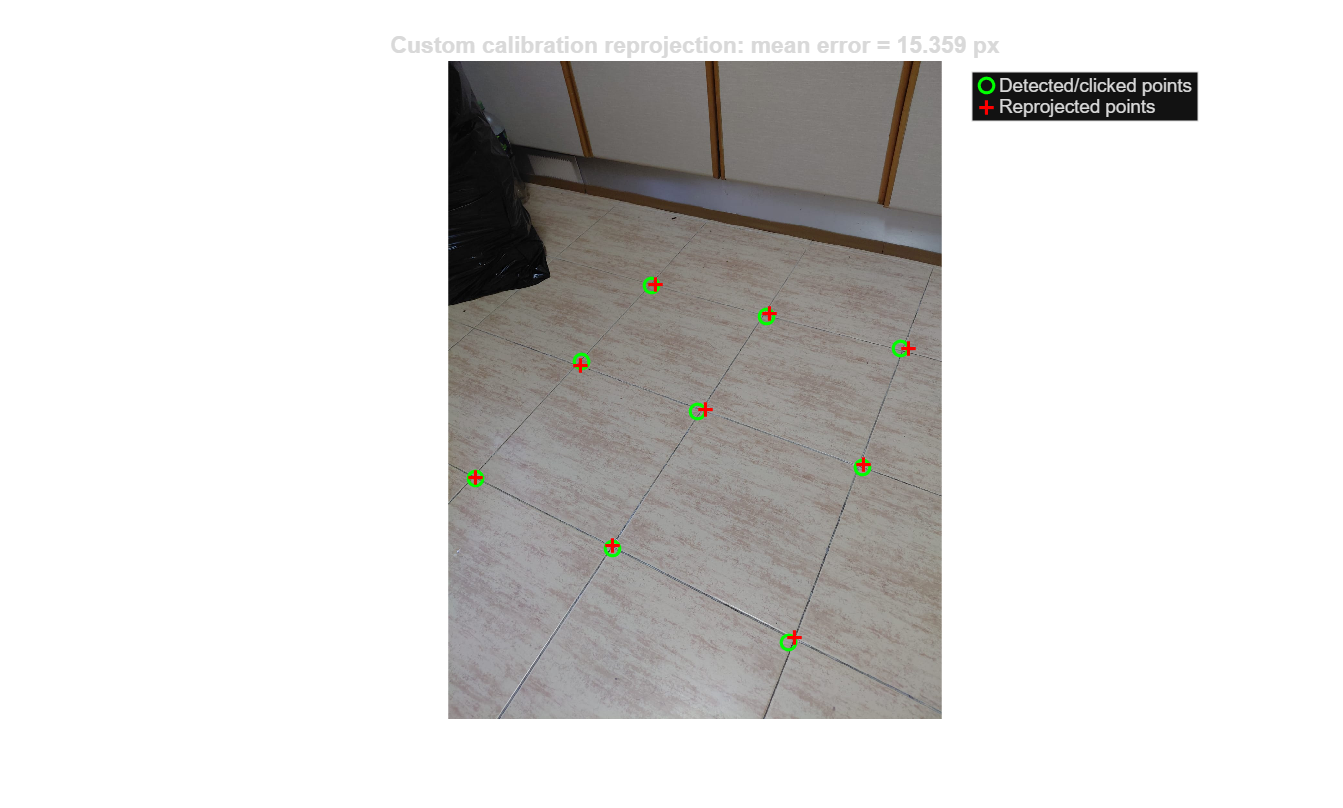
\includegraphics[width=0.75\textwidth]{section_1/reprojection_custom.png}
    \caption{Reprojection check for custom floor-tile calibration:
             detected (clicked) corners (green circles) vs.\ reprojected corners
             (red crosses) on image~1.  Mean reprojection error:
             $15.359\,\mathrm{px}$.}
    \label{fig:reproj_custom}
\end{figure}

The mean reprojection error is $15.359\,\mathrm{px}$, approximately $1.57\times$
larger than the screen value.  The higher error reflects three compounding
sources of uncertainty: (i)~click imprecision in localising the grout-line
intersections, (ii)~perspective-induced foreshortening near the image
boundaries that makes point identification less precise, and (iii)~the
limited number of points (9 per image versus 64 for the screen board),
which provides less algebraic redundancy for the homography fit.

% ------------------------------------------------------------
\subsection{Comparison Between \texorpdfstring{$\mathbf{A}$}{A} and
            \texorpdfstring{$\mathbf{A}'$}{A'}}
\label{sec:comparison}
% ------------------------------------------------------------

\subsubsection*{Theoretical expectation}

Because $\mathbf{A}$ and $\mathbf{A}'$ were estimated from the same physical
camera with all internal settings fixed (focal length, zoom, aperture, and
aspect ratio unchanged between sessions), they should in theory represent the
same intrinsic parameter set.  The ideal intrinsic matrix is a fixed property
of the optical system: it does not depend on the calibration pattern used, the
scene, or the viewpoints, provided the imaging geometry is correctly modelled.
A well-conditioned calibration should therefore yield $\mathbf{A} \approx \mathbf{A}'$.

\subsubsection*{Practical differences and their causes}

Table~\ref{tab:comparison} quantifies the discrepancy between the two matrices.

\begin{table}[htbp]
\centering
\caption{Comparison between screen-checkerboard calibration $\mathbf{A}$ and
         custom floor-tile calibration $\mathbf{A}'$.}
\label{tab:comparison}
\begin{tabular}{lr}
\hline
Metric & {Value} \\
\hline
Frobenius norm $\|\mathbf{A} - \mathbf{A}'\|_F$  & 451.298421 \\
$\alpha$ percent difference [\%]                   & 16.596577  \\
$\beta$ percent difference [\%]                    & 13.284514  \\
$u_0$ difference [px]                              & -58.012671 \\
$v_0$ difference [px]                              & 305.570924 \\
Skew difference [px]                               & -35.766142 \\
Aspect-ratio difference                            & -0.029300  \\
\hline
\end{tabular}
\end{table}

The Frobenius norm $\|\mathbf{A}-\mathbf{A}'\|_F = 451.30$ indicates a
substantial absolute difference, driven primarily by the large vertical
principal-point discrepancy ($\Delta v_0 = 305.57\,\mathrm{px}$) and the
focal-length discrepancies of $16.6\%$ in $\alpha$ and $13.3\%$ in $\beta$.
Several factors explain why the custom calibration deviates more from
the true intrinsics:

\begin{enumerate}
    \item \textbf{Point density.}  The screen checkerboard provides 64 automatically
          detected sub-pixel-accurate corners per image.  The floor-tile pattern
          provides only 9 manually clicked corners, giving far fewer constraints
          on the homography and consequently on the intrinsic parameters.
    \item \textbf{Localisation precision.}  Automatic corner detection on a
          high-contrast printed (or displayed) checkerboard achieves sub-pixel
          accuracy.  Manual clicking on grout-line intersections introduces
          random errors of several pixels, which directly propagate into the
          homography estimates.
    \item \textbf{Pattern extent and diversity.}  The screen checkerboard covers a
          large image area with corners distributed densely and uniformly,
          providing good coverage of the distortion field.  The $3\times3$
          floor-tile grid spans only 9 widely spaced points, limiting the
          observability of off-axis lens behaviour.
    \item \textbf{Perspective distortion.}  The floor tiles were captured at
          oblique angles to introduce viewpoint diversity; however, at steep
          angles the foreshortened grout lines are harder to localise accurately.
    \item \textbf{Lens distortion and lighting.}  Radial lens distortion shifts
          the apparent position of points near the image borders, an effect that
          is partially absorbed into the homography parameters when the model
          does not explicitly account for distortion.
\end{enumerate}

\subsubsection*{Conclusion}

Given the substantially lower reprojection error ($9.764\,\mathrm{px}$ vs.\
$15.359\,\mathrm{px}$), the much smaller principal-point offset ($5.13\%$
vs.\ $19.38\%$ of the half-diagonal), the nearly unity aspect ratio
($0.218\%$ deviation vs.\ $3.148\%$), and the denser, automatically detected
point correspondences, the screen-checkerboard intrinsic matrix $\mathbf{A}$
(Eq.~\eqref{eq:A_screen}) is considered more reliable.
Accordingly, $\mathbf{A}$ will be used as the camera intrinsic matrix in
Sections~2 and~3 of this report.

% ============================================================
\section{Finding Local Matches Between Several Views of an Object}
% ============================================================

This section presents the scene acquisition, feature detection and matching experiments across five representative image pairs and four detector/descriptor setups, a per-octave SIFT analysis, and the selection of the best combination for Section~3.

% ------------------------------------------------------------
\subsection{Scene Capture and Image Scaling}
\label{sec:scene_capture}
% ------------------------------------------------------------

Five portrait-orientation views (View\_01--View\_05.jpeg, $1530 \times 2040\,\mathrm{px}$)
were captured with the calibrated camera from Section~\ref{sec:screen_calib}.
For computational efficiency each image was uniformly downscaled by
$s = 0.66928105$ to $1024 \times 1366\,\mathrm{px}$.
Per LabFinal Note~2, downscaling requires updating the intrinsic matrix: the first two
rows of $\mathbf{A}$ are multiplied by $s$, while $K_{3,3}=1$ is unchanged.
The resulting scaled matrix is:

\begin{equation}
\mathbf{A}_\mathrm{sc} =
\begin{bmatrix}
1024.194411 & -9.305537 & 512.039937 \\
0           & 1021.971110 & 726.456479 \\
0           & 0           & 1
\end{bmatrix}
\label{eq:A_scaled}
\end{equation}

Figure~\ref{fig:section2_scene_montage} shows the five captured views.

\begin{figure}[!htbp]
    \centering
    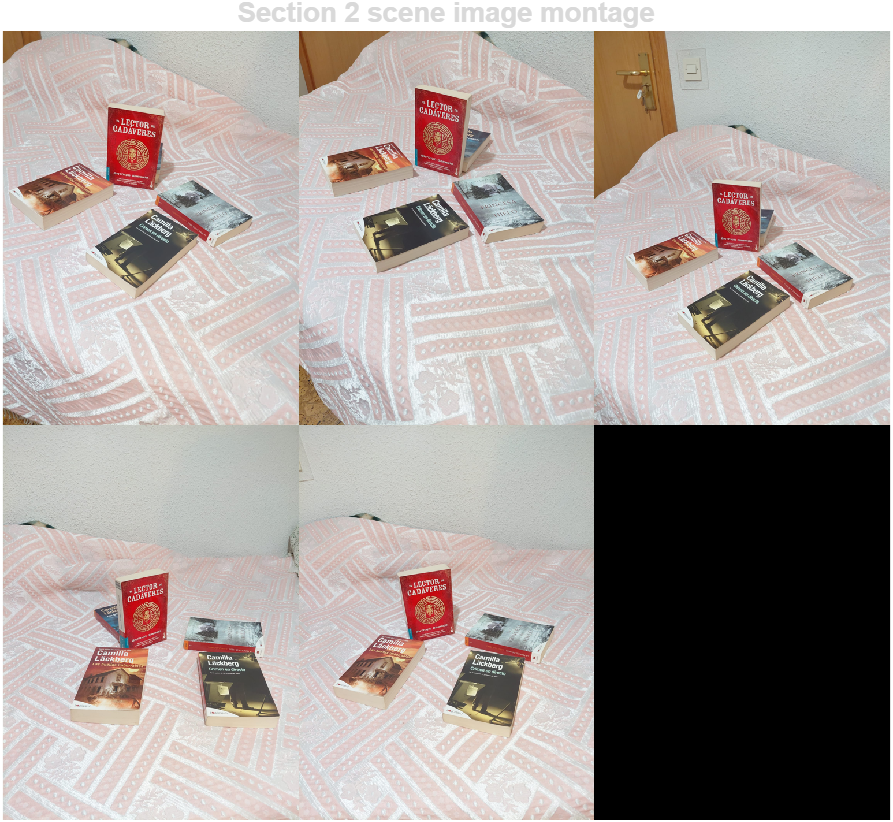
\includegraphics[width=0.62\textwidth]{section_2/scene_montage.png}
    \caption{Montage of the five scene views (View\_01 to View\_05) captured with
             the calibrated camera.}
    \label{fig:section2_scene_montage}
\end{figure}

The scene consists of four books arranged on a textured bedsheet.
Challenging factors include: non-planar depth variation between the books
(a planar homography is only an approximation for any pair), repetitive
low-contrast texture on the bedsheet (susceptible to false matches),
partial book occlusions between views, and specular reflections on book covers
that shift the apparent position of keypoints.

% ------------------------------------------------------------
\subsection{Feature Detection, Description, and Matching Setups}
\label{sec:sec2_setups}
% ------------------------------------------------------------

Five pairs spanning short to wide baselines were selected: V01--V02 and V02--V03
(adjacent, high overlap), V01--V03 (medium), V03--V05 (medium/wide), and
V01--V05 (widest).  Four setups were evaluated: SIFT-D, SIFT-S, SURF, and ORB.
SIFT-D used the default MATLAB SIFT configuration; SIFT-S used stricter matching
parameters; SURF and ORB used MATLAB feature extraction with descriptor matching.
For every combination, a homography $\mathbf{H}$ and a fundamental matrix
$\mathbf{F}$ were estimated with RANSAC.

% ------------------------------------------------------------
\subsection{Quantitative Comparison of Matching Setups}
\label{sec:sec2_comparison}
% ------------------------------------------------------------

The full 20-row comparison is stored in
\path{results/section_2/setup_comparison.csv}.  To keep the report concise,
Table~\ref{tab:section2_four_setup_comparison} gives a direct comparison of all
four setups on the selected best image pair, View\_02.jpeg vs View\_03.jpeg.

\begin{table}[htbp]
\centering
\caption{Detector/descriptor comparison for View\_02.jpeg vs View\_03.jpeg.}
\label{tab:section2_four_setup_comparison}
\begin{tabular}{lrrrrr}
\hline
Setup & Matches & H inl. & H res. & F inl. & F err. \\
\hline
SIFT MATLAB default & 955  & 326 & 0.500576 & 703 & 0.110435 \\
SIFT MATLAB strict  & 1003 & 306 & 0.709384 & 714 & 0.183218 \\
SURF matchFeatures  & 304  & 183 & 1.649812 & 185 & 0.389158 \\
ORB matchFeatures   & 390  & 251 & 0.990057 & 301 & 0.139163 \\
\hline
\end{tabular}
\end{table}

For the selected best pair, both SIFT variants produced many more
$\mathbf{F}$ inliers than SURF and ORB.  ORB was competitive in speed and had a
low Sampson error, but it produced fewer reliable correspondences than SIFT.
SURF produced fewer matches and a higher homography residual on this scene.  The
strict SIFT setup was selected because it gave the largest number of
$\mathbf{F}$ inliers, which is the most important criterion for the later 3D
reconstruction stage.  The homography residual grows with baseline, confirming
non-negligible scene depth; $\mathbf{F}$ is therefore the more appropriate
geometric model for reconstruction.

Table~\ref{tab:section2_top_combinations} lists the four best combinations, ranked by
$\mathbf{F}$ inlier count.  Two pairs account for all four top slots:
V02--V03 (adjacent, high overlap) and V01--V03 (medium baseline).

\begin{table}[htbp]
\centering
\caption{Top four pair/setup combinations ranked by fundamental matrix inlier count.}
\label{tab:section2_top_combinations}
\begin{tabular}{llrrrr}
\hline
Pair     & Setup  & {F inl.} & {F err.} & {H inl.} & {H res.} \\
\hline
V02--V03 & SIFT-S & 714 & 0.183218 & 306 & 0.709384 \\
V02--V03 & SIFT-D & 703 & 0.110435 & 326 & 0.500576 \\
V01--V03 & SIFT-S & 638 & 0.253738 & 347 & 1.116479 \\
V01--V03 & SIFT-D & 625 & 0.156698 & 388 & 1.313458 \\
\hline
\end{tabular}
\end{table}

% ------------------------------------------------------------
\subsection{Per-Octave SIFT Experiment}
\label{sec:sec2_octave}
% ------------------------------------------------------------

The best pair (V02--V03) was re-evaluated restricting keypoints to individual SIFT octave
groups to assess scale-level contributions.
Table~\ref{tab:section2_octave_summary} and Figure~\ref{fig:section2_octave} summarise
the results; Figure~\ref{fig:section2_octave} also shows correspondences restricted to
Octave~0 (the dominant scale level).

\begin{table}[htbp]
\centering
\caption{Per-octave SIFT results for V02--V03. KP = keypoints detected per image.
         $\infty$ = too few inliers for a reliable $\mathbf{F}$ estimate.}
\label{tab:section2_octave_summary}
\begin{tabular}{rlrrrr}
\hline
Oct.  & KP1/KP2   & {Matches} & {H inl.} & {F inl.} & {F err.} \\
\hline
$-1$  & 484/570   & 85  & 23  & 40  & 0.086550 \\
$0$   & 1477/1448 & 541 & 208 & 402 & 0.229498 \\
$1$   & 369/352   & 121 & 69  & 79  & 0.511258 \\
$2$   & 164/156   & 65  & 39  & 43  & 0.193750 \\
$3$   & 60/45     & 26  & 18  & 18  & 0.369026 \\
$4$   & 17/20     & 11  & 6   & 9   & 0.036851 \\
$5$   & 3/5       & 2   & 0   & 0   & {$\infty$} \\
$6$   & 5/4       & 3   & 0   & 0   & {$\infty$} \\
\hline
\end{tabular}
\end{table}

% NOTE: Generate octave0_matches.png by saving a correspondence figure restricted to
% Octave 0 in Roy_Gourab_2.m, then copy it to latex_report/images/section_2/
\begin{figure}[htbp]
    \centering
    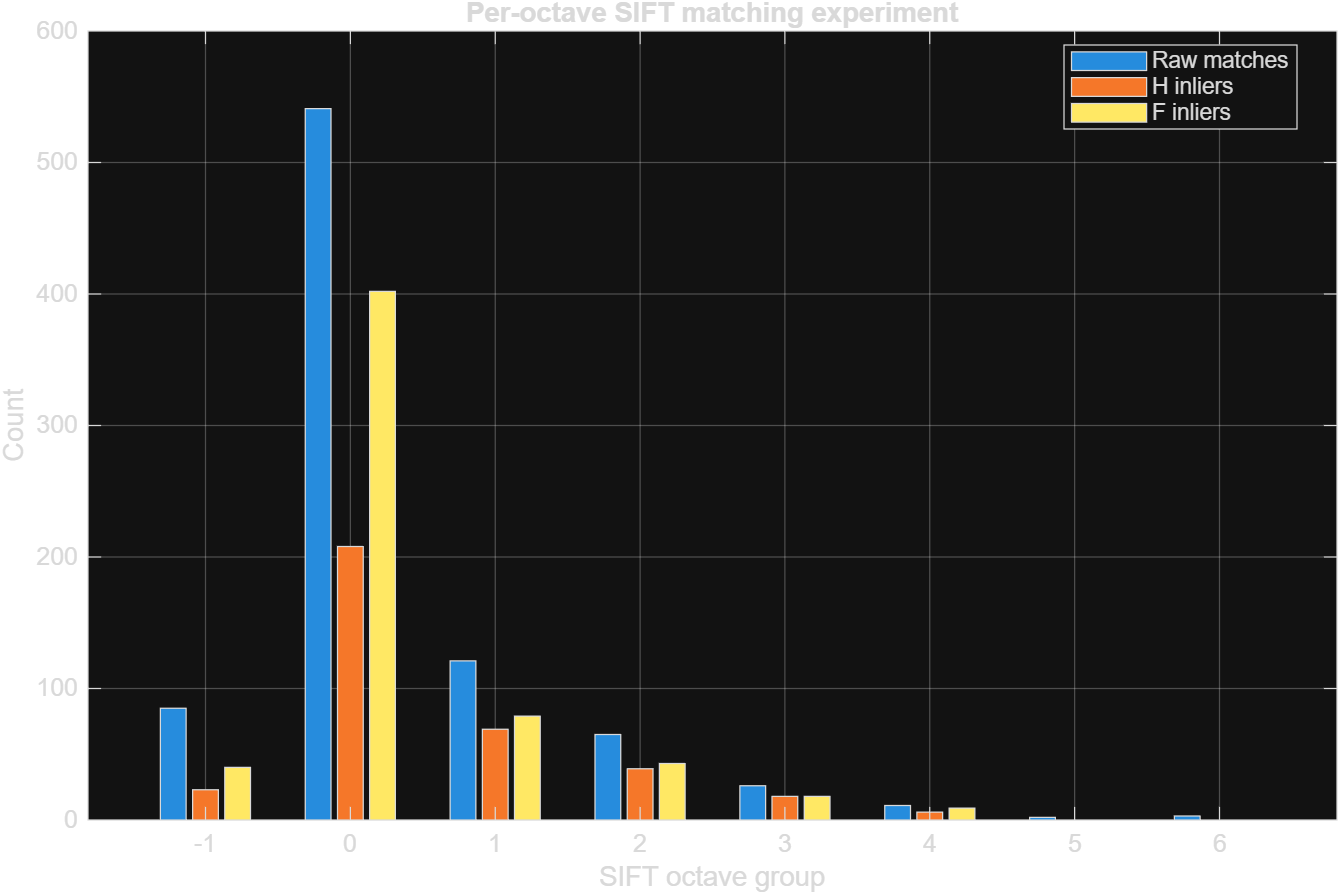
\includegraphics[width=0.54\textwidth]{section_2/per_octave_results.png}
    \hfill
    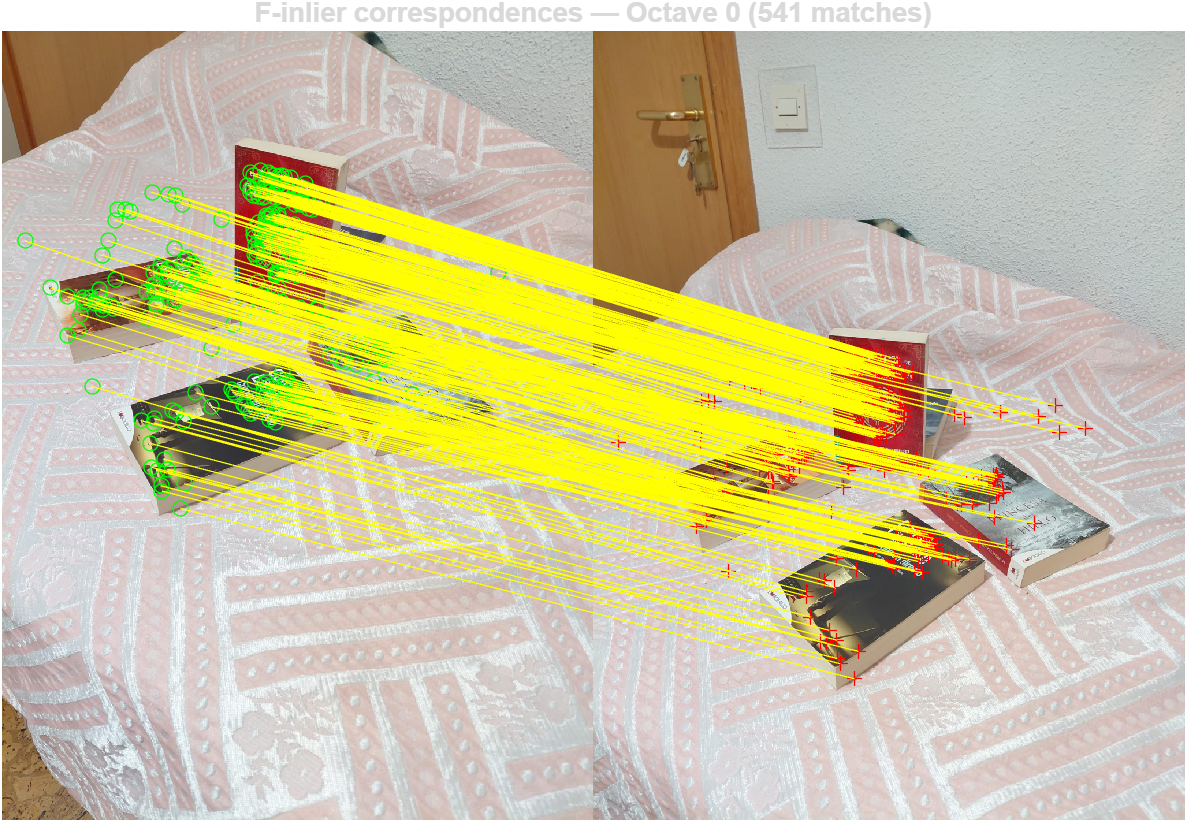
\includegraphics[width=0.44\textwidth]{section_2/octave0_matches.png}
    \caption{Left: per-octave match/inlier counts for V02--V03 ($\mathbf{H}$ and
             $\mathbf{F}$ inliers).  Right: F-inlier correspondences restricted to
             Octave~0 (541 raw matches, 402~$\mathbf{F}$ inliers).}
    \label{fig:section2_octave}
\end{figure}

Octave~0 dominates with 541 of 1003 full-detector matches; octaves~5--6 are too sparse
for reliable estimation.
\textbf{Advantages:} isolates scale-specific structures; suppresses cross-scale false
matches.
\textbf{Drawbacks:} discards the majority of valid correspondences; high octaves provide
insufficient points for robust $\mathbf{F}$ estimation; the full-detector output is more
stable than any single octave slice.

% ------------------------------------------------------------
\subsection{Best Combination and Geometric Outputs}
\label{sec:sec2_best}
% ------------------------------------------------------------

Based on Tables~\ref{tab:section2_four_setup_comparison} and
\ref{tab:section2_top_combinations}, the
best combination is \textbf{View\_02 vs View\_03 with SIFT MATLAB strict}:
1003 raw matches, 714 $\mathbf{F}$~inliers ($71.2\%$), Sampson error $0.183218$,
306 $\mathbf{H}$~inliers ($30.5\%$), homography residual $0.709384\,\mathrm{px}$.
Figure~\ref{fig:section2_best_matches} shows the inlier correspondences.

\begin{figure}[!htbp]
    \centering
    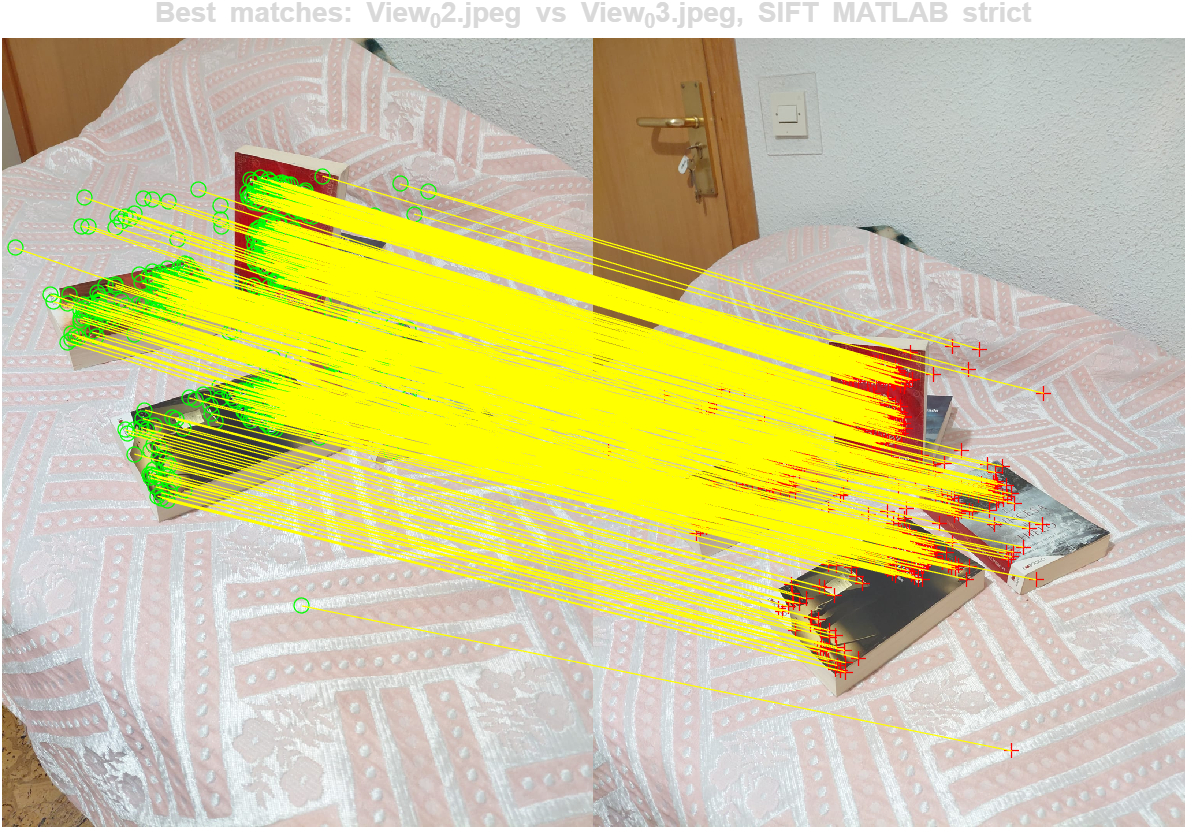
\includegraphics[width=0.86\textwidth]{section_2/best_matches.png}
    \caption{Fundamental matrix inlier correspondences for the best combination
             (View\_02 vs View\_03, SIFT MATLAB strict).
             Green circles: keypoints in View\_02;
             red crosses: matched keypoints in View\_03.}
    \label{fig:section2_best_matches}
\end{figure}

\subsubsection*{Homography, fundamental matrix, and geometric verification}

The homography from View\_02 to View\_03 is:

\begin{equation}
\mathbf{H} =
\begin{bmatrix}
 1.288474 & -0.052662 & -49.841671 \\
 0.153312 &  0.769757 & 380.728394 \\
 0.000446 & -0.000249 &   1.000000
\end{bmatrix}
\label{eq:sec2_H}
\end{equation}

The estimated fundamental matrix ($\mathbf{F}$ rank-2, unit Frobenius norm) is:

\begin{equation}
\mathbf{F} =
\begin{bmatrix}
 0.000000 &  0.000001 &  0.000183 \\
-0.000001 &  0.000000 & -0.002453 \\
 0.000032 &  0.001922 &  0.999995
\end{bmatrix}
\label{eq:sec2_F}
\end{equation}

Figure~\ref{fig:sec2_pano_vgg} shows the panorama obtained with $\mathbf{H}$
and the \texttt{vgg\_gui\_F.m} screenshot used to inspect the epipolar geometry.

\begin{figure}[!htbp]
    \centering
    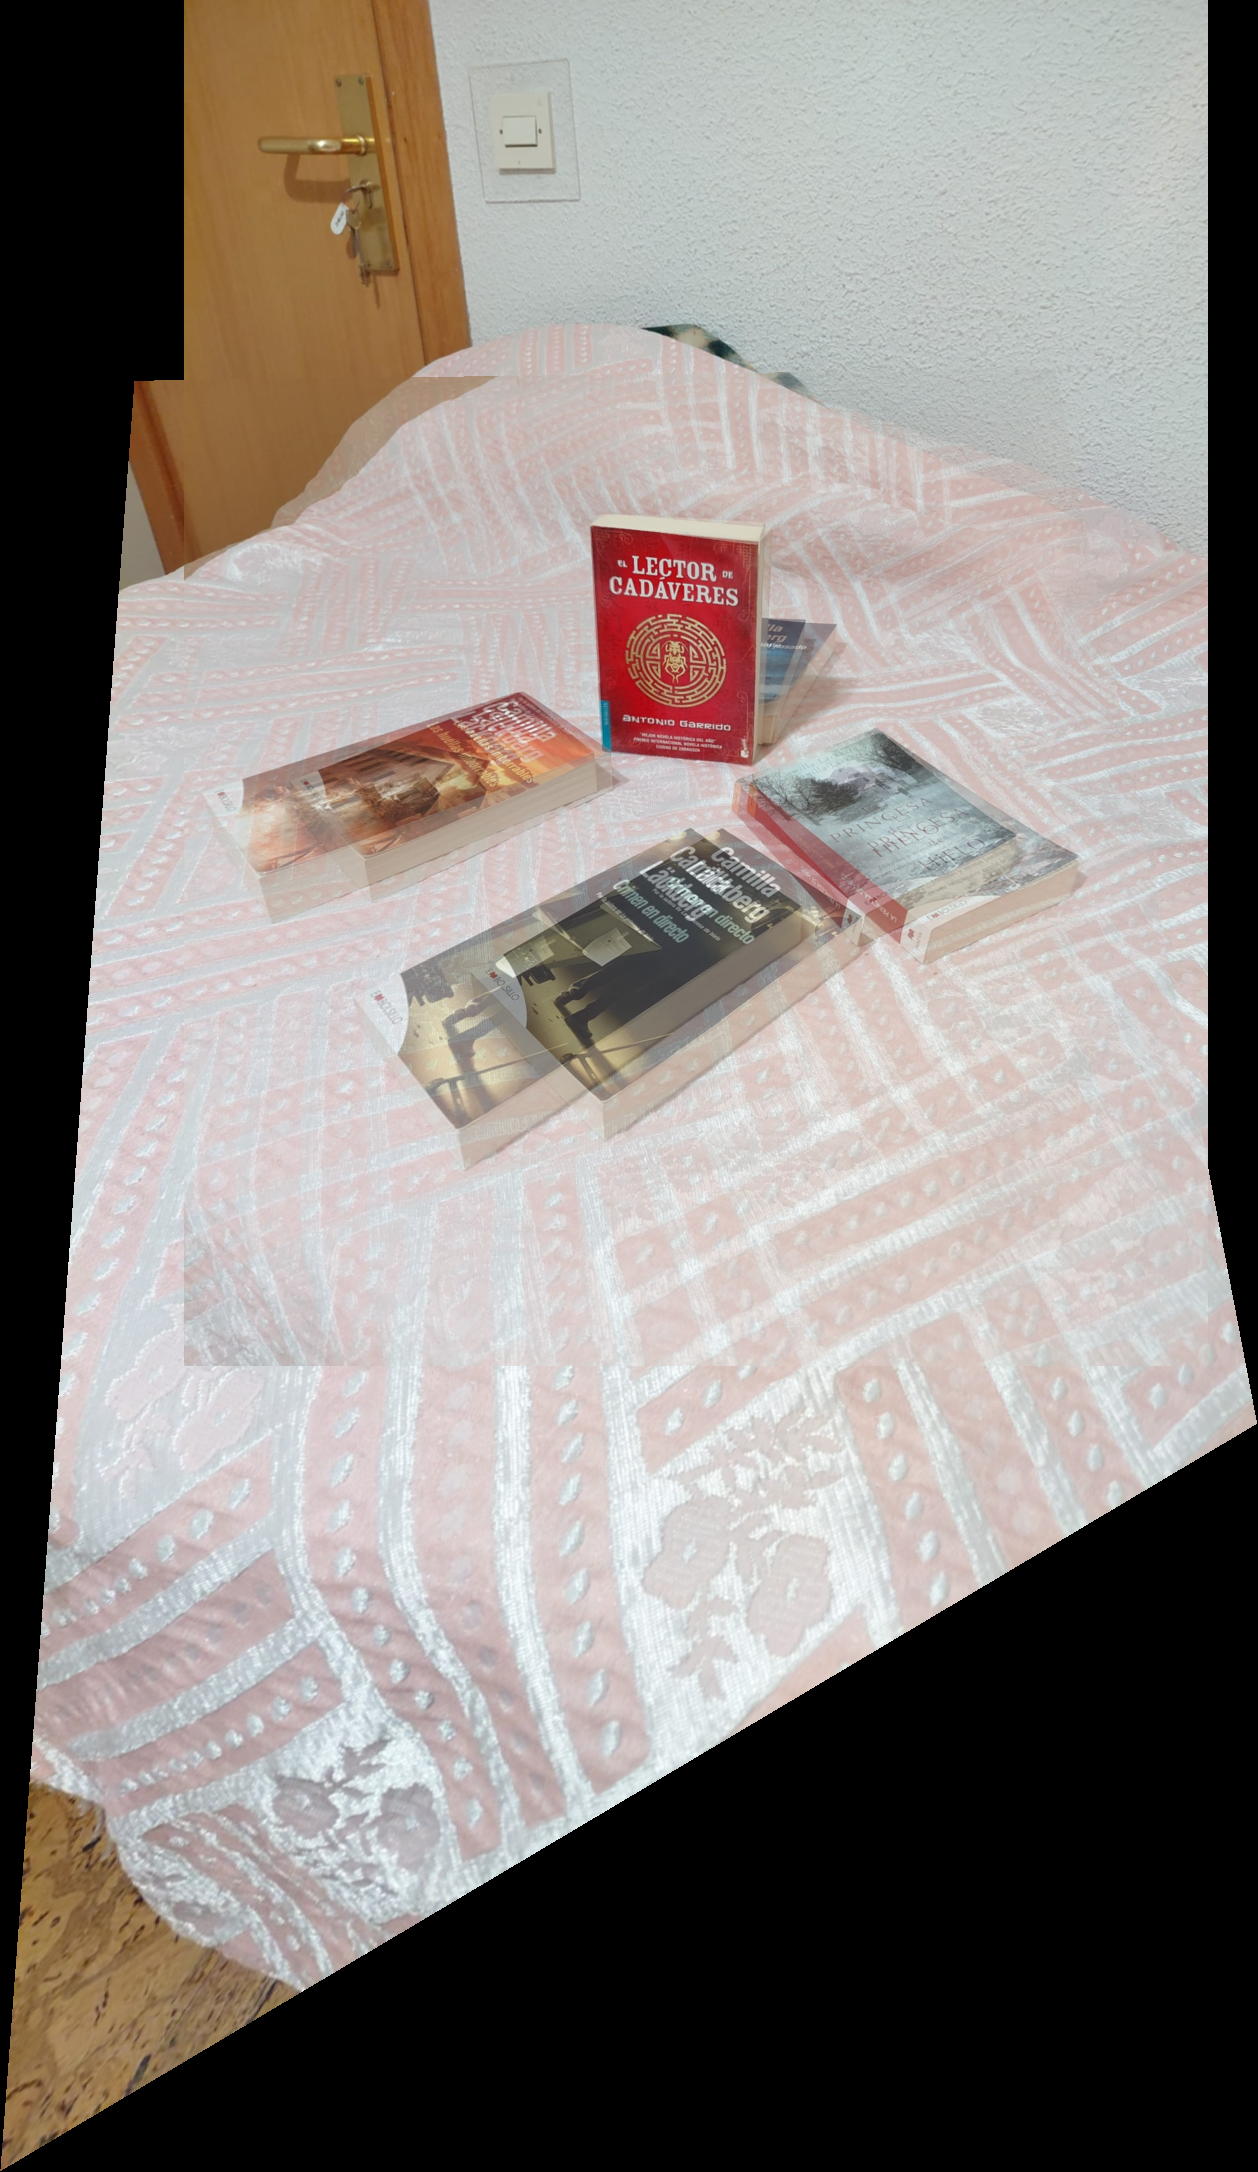
\includegraphics[height=0.30\textheight]{section_2/best_panorama.png}
    \hfill
    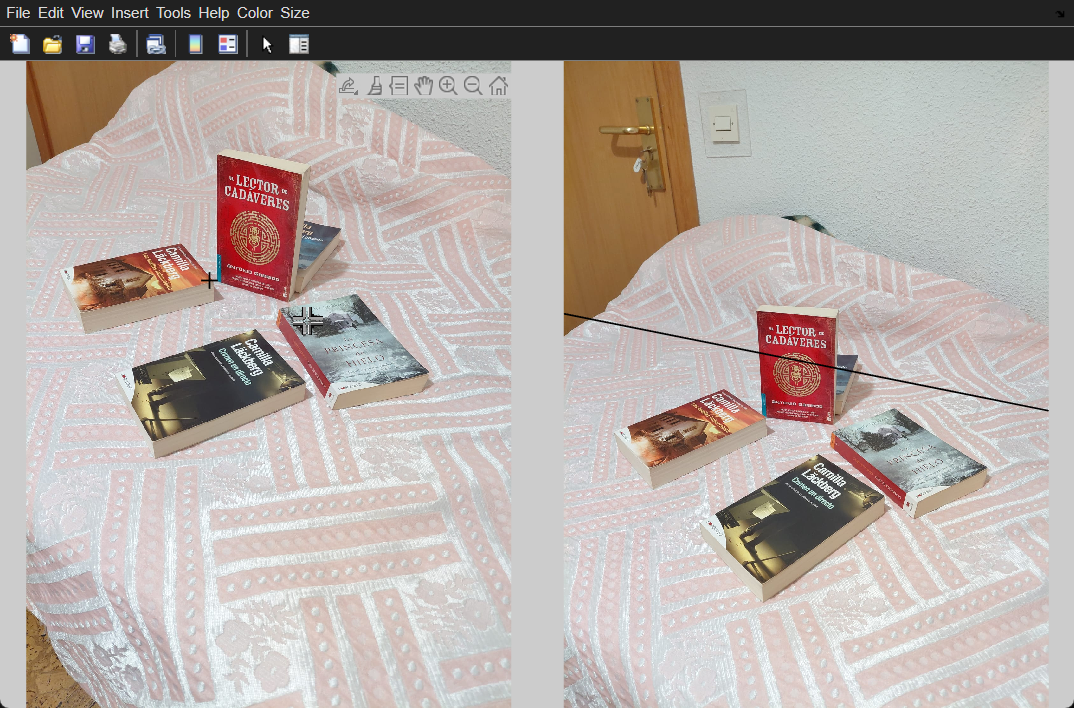
\includegraphics[height=0.30\textheight]{section_2/vgg_gui_F_best_pair_screenshot.png}
    \caption{Left: panorama warping View\_02 onto View\_03 via $\mathbf{H}$
             (Eq.~\eqref{eq:sec2_H}).
             Right: \texttt{vgg\_gui\_F.m} GUI -- a selected point in the left image
             generates its epipolar line in the right image, confirming
             $\mathbf{F}$ quality (Eq.~\eqref{eq:sec2_F}).}
    \label{fig:sec2_pano_vgg}
\end{figure}

\clearpage

% ============================================================
\section{3D Reconstruction from Multiple Views}
% ============================================================

This section describes the complete pipeline for recovering a Euclidean 3D point cloud
from five calibrated views: N-view track building, initial two-camera projective
reconstruction, resectioning of the remaining cameras, projective bundle adjustment,
and final Euclidean factorisation via the Essential matrix.

% ------------------------------------------------------------
\subsection{N-View Keypoint Detection and Track Building}
\label{sec:sec3_nview}
% ------------------------------------------------------------

The N-view reconstruction used five images: View\_01.jpeg through
View\_05.jpeg.  MATLAB SIFT (\texttt{detectSIFTFeatures}) was applied to each
of the five scaled views ($1024 \times 1366\,\mathrm{px}$).
Table~\ref{tab:sec3_keypoints} lists the keypoint counts.  Figures~\ref{fig:sec3_kp_01_02}
and~\ref{fig:sec3_kp_03_05} show the detected SIFT interest points for all five
views used in the N-view matching stage.

\begin{table}[htbp]
\centering
\caption{SIFT keypoint counts per view and N-view track statistics.}
\label{tab:sec3_keypoints}
\begin{tabular}{lr}
\hline
Item & Value \\
\hline
View\_01.jpeg & 2576 keypoints \\
View\_02.jpeg & 2579 keypoints \\
View\_03.jpeg & 2600 keypoints \\
View\_04.jpeg & 2685 keypoints \\
View\_05.jpeg & 2699 keypoints \\
\hline
Tracks retained (N-view) & 672 \\
Reference view          & View\_03.jpeg \\
Min.\ track visibility  & 2 views \\
Max.\ track visibility  & 5 views \\
Mean track visibility   & 3.107 views \\
\hline
\end{tabular}
\end{table}

\begin{figure}[htbp]
    \centering
    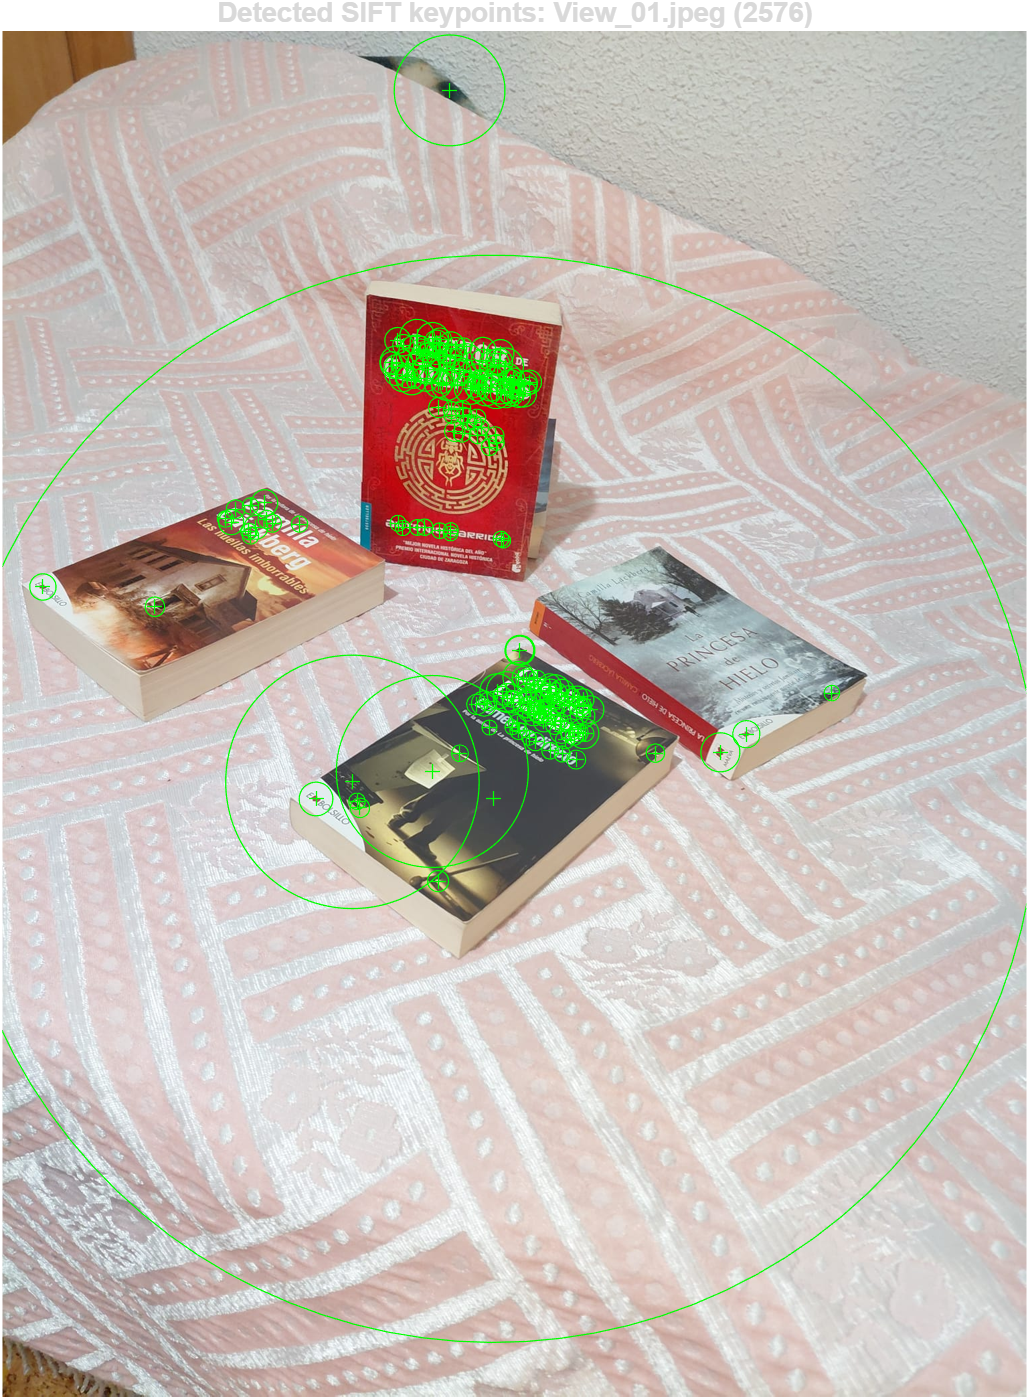
\includegraphics[width=0.48\textwidth]{section_3/keypoints_view_01.png}
    \hfill
    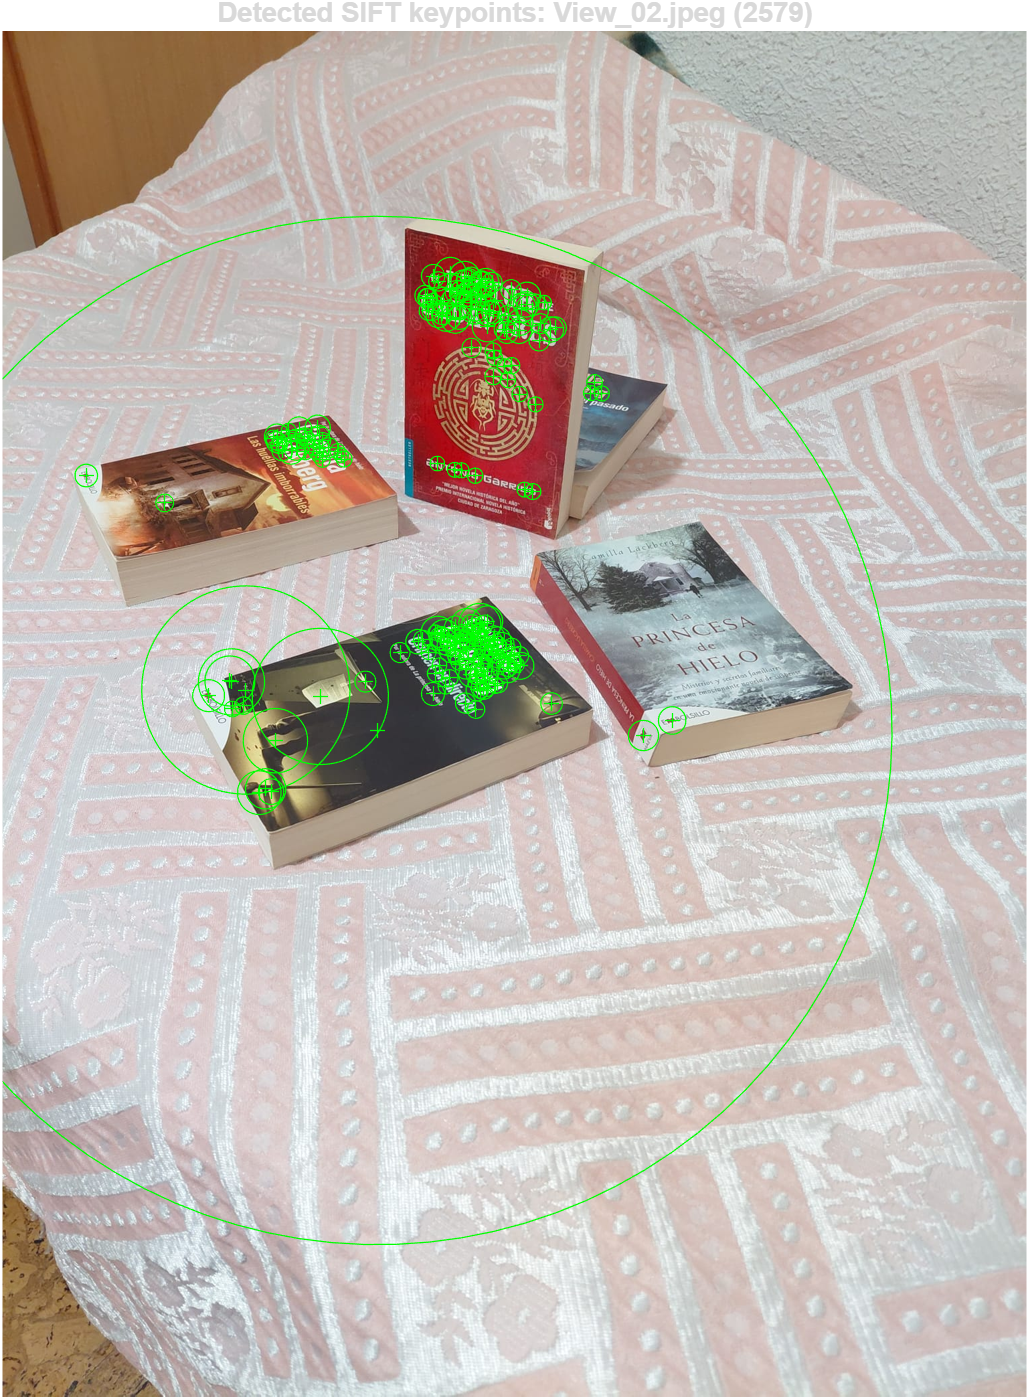
\includegraphics[width=0.48\textwidth]{section_3/keypoints_view_02.png}
    \caption{SIFT keypoints detected in the first two N-view matching images:
             View\_01.jpeg (left, 2576 keypoints) and View\_02.jpeg
             (right, 2579 keypoints).}
    \label{fig:sec3_kp_01_02}
\end{figure}

\begin{figure}[htbp]
    \centering
    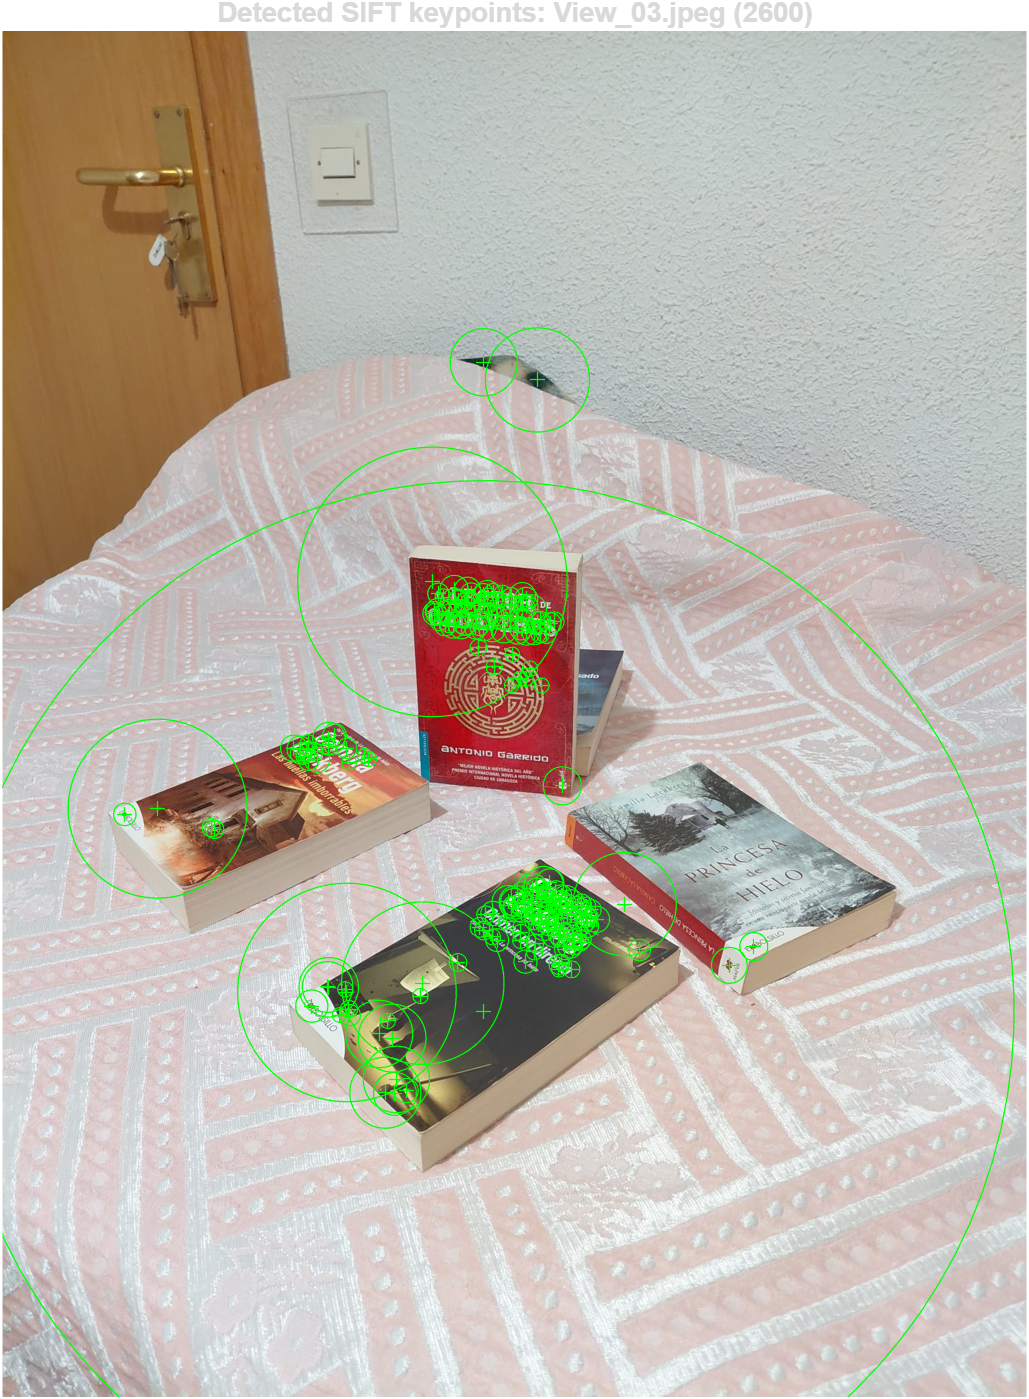
\includegraphics[width=0.32\textwidth]{section_3/keypoints_view_03.png}
    \hfill
    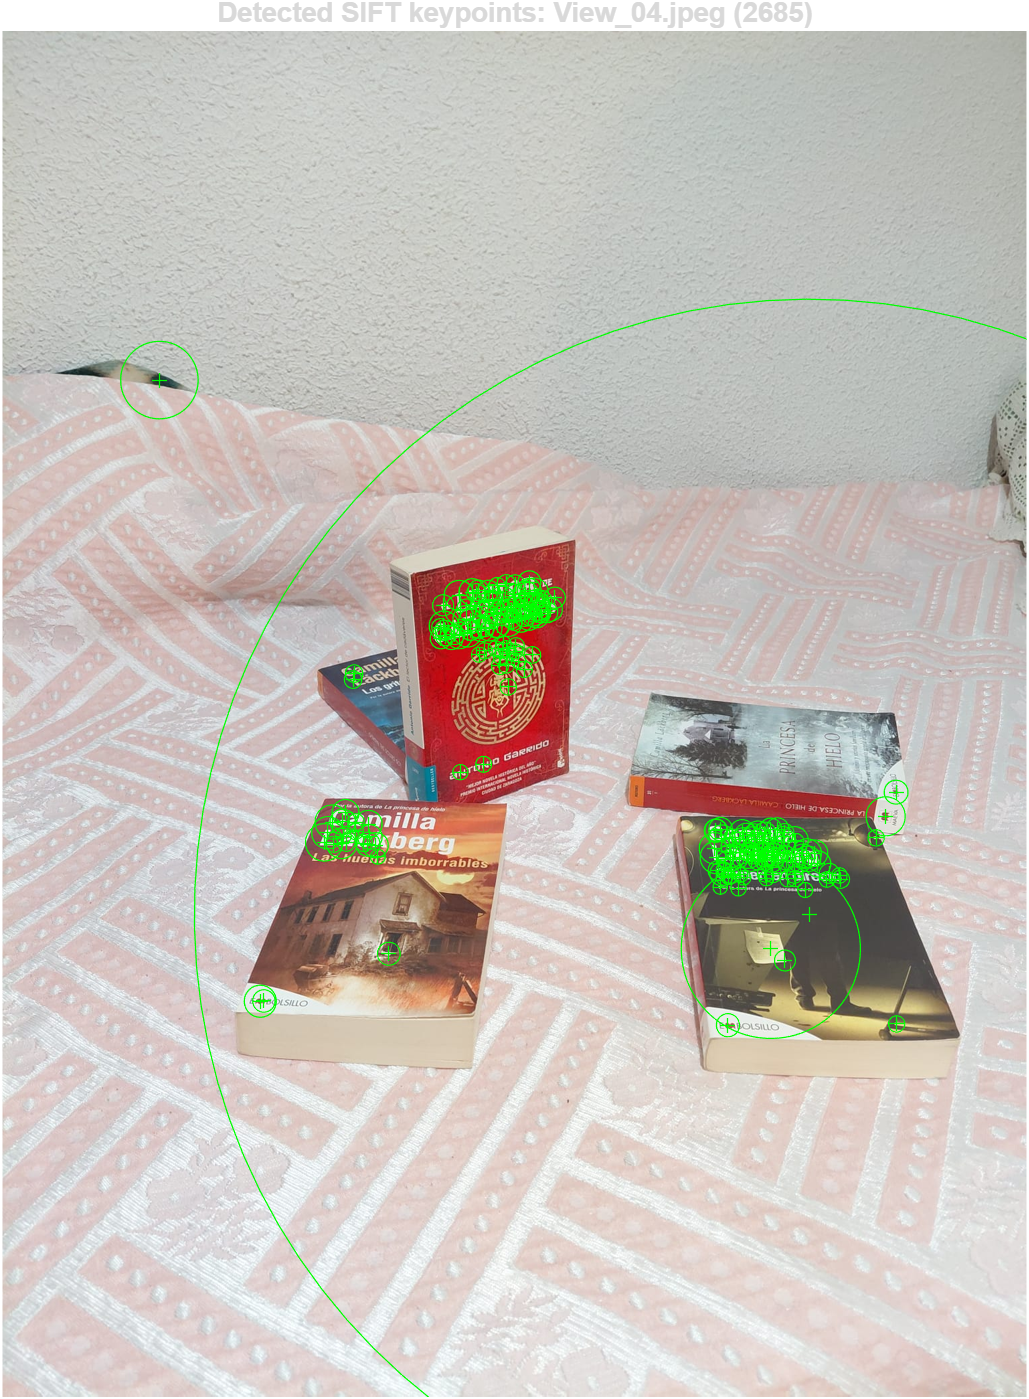
\includegraphics[width=0.32\textwidth]{section_3/keypoints_view_04.png}
    \hfill
    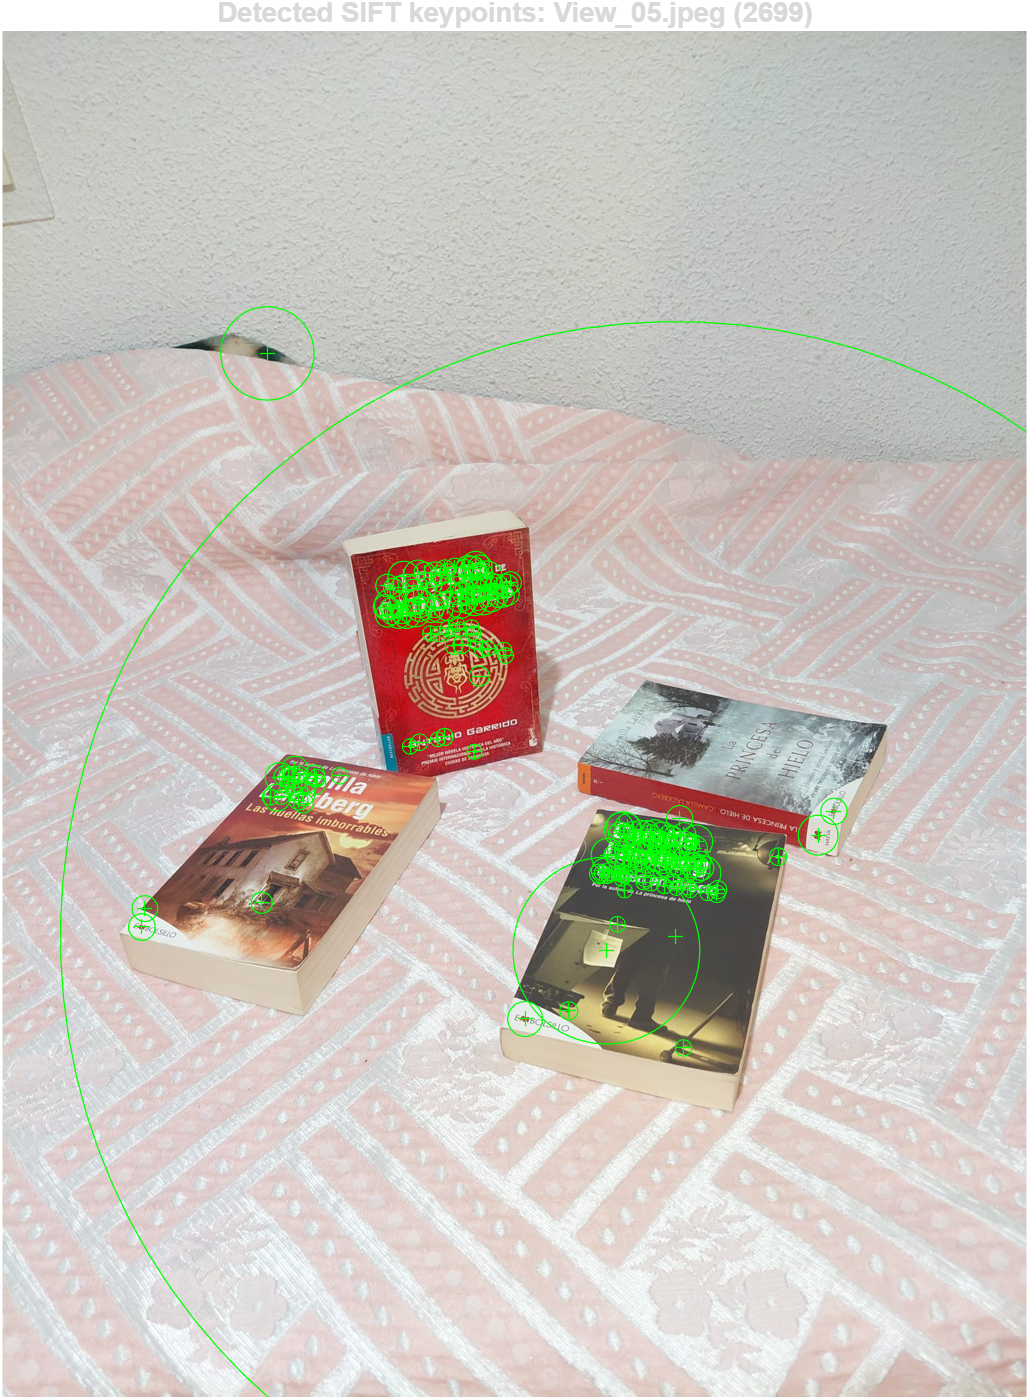
\includegraphics[width=0.32\textwidth]{section_3/keypoints_view_05.png}
    \caption{SIFT keypoints in View\_03.jpeg, the reference view
             (left, 2600 keypoints), View\_04.jpeg (centre, 2685 keypoints),
             and View\_05.jpeg (right, 2699 keypoints).}
    \label{fig:sec3_kp_03_05}
\end{figure}

N-view tracks were built using a reference-view strategy.  The middle view,
View\_03.jpeg, was selected as the reference because it provides strong overlap
with neighbouring views.  Each remaining view was matched against the reference
view, and the matches were filtered using fundamental-matrix RANSAC before being
kept as multi-view tracks.  Of the initial detections, 672 tracks survived this
filtering stage.  The mean visibility of $3.107$ views per track indicates that
most 3D points are visible in three or more images, providing good redundancy
for reconstruction.

% ------------------------------------------------------------
\subsection{Initial Two-Camera Projective Reconstruction}
\label{sec:sec3_initial}
% ------------------------------------------------------------

The initial projective reconstruction used the best pair from Section~2
(\textbf{View\_02 vs View\_03}).
RANSAC fundamental matrix estimation on 734 pair tracks yielded 672 inliers
(mean reprojection error $0.169020\,\mathrm{px}$).
The initial fundamental matrix is:

\begin{equation}
\mathbf{F}_0 =
\begin{bmatrix}
 0.00000003 & -0.00000001 &  0.00021335 \\
-0.00000039 &  0.00000043 & -0.00242889 \\
-0.00028406 &  0.00174221 &  0.99999547
\end{bmatrix}
\label{eq:sec3_F0}
\end{equation}

The canonical projective camera pair was set as
$\mathbf{P}_1 = [\mathbf{I}\,|\,\mathbf{0}]$ and
$\mathbf{P}_2 = [\mathbf{A}\,|\,\mathbf{b}]$ derived from
$\mathbf{F}_0$ via the epipole decomposition.
The 3D points were triangulated by DLT and an initial point cloud
of 672 structure points was obtained.

Figure~\ref{fig:sec3_initial_matches} shows the inlier correspondences on the
initial pair, and Figure~\ref{fig:sec3_initial_hist} shows the reprojection error
histogram after initial reconstruction.

\begin{figure}[htbp]
    \centering
    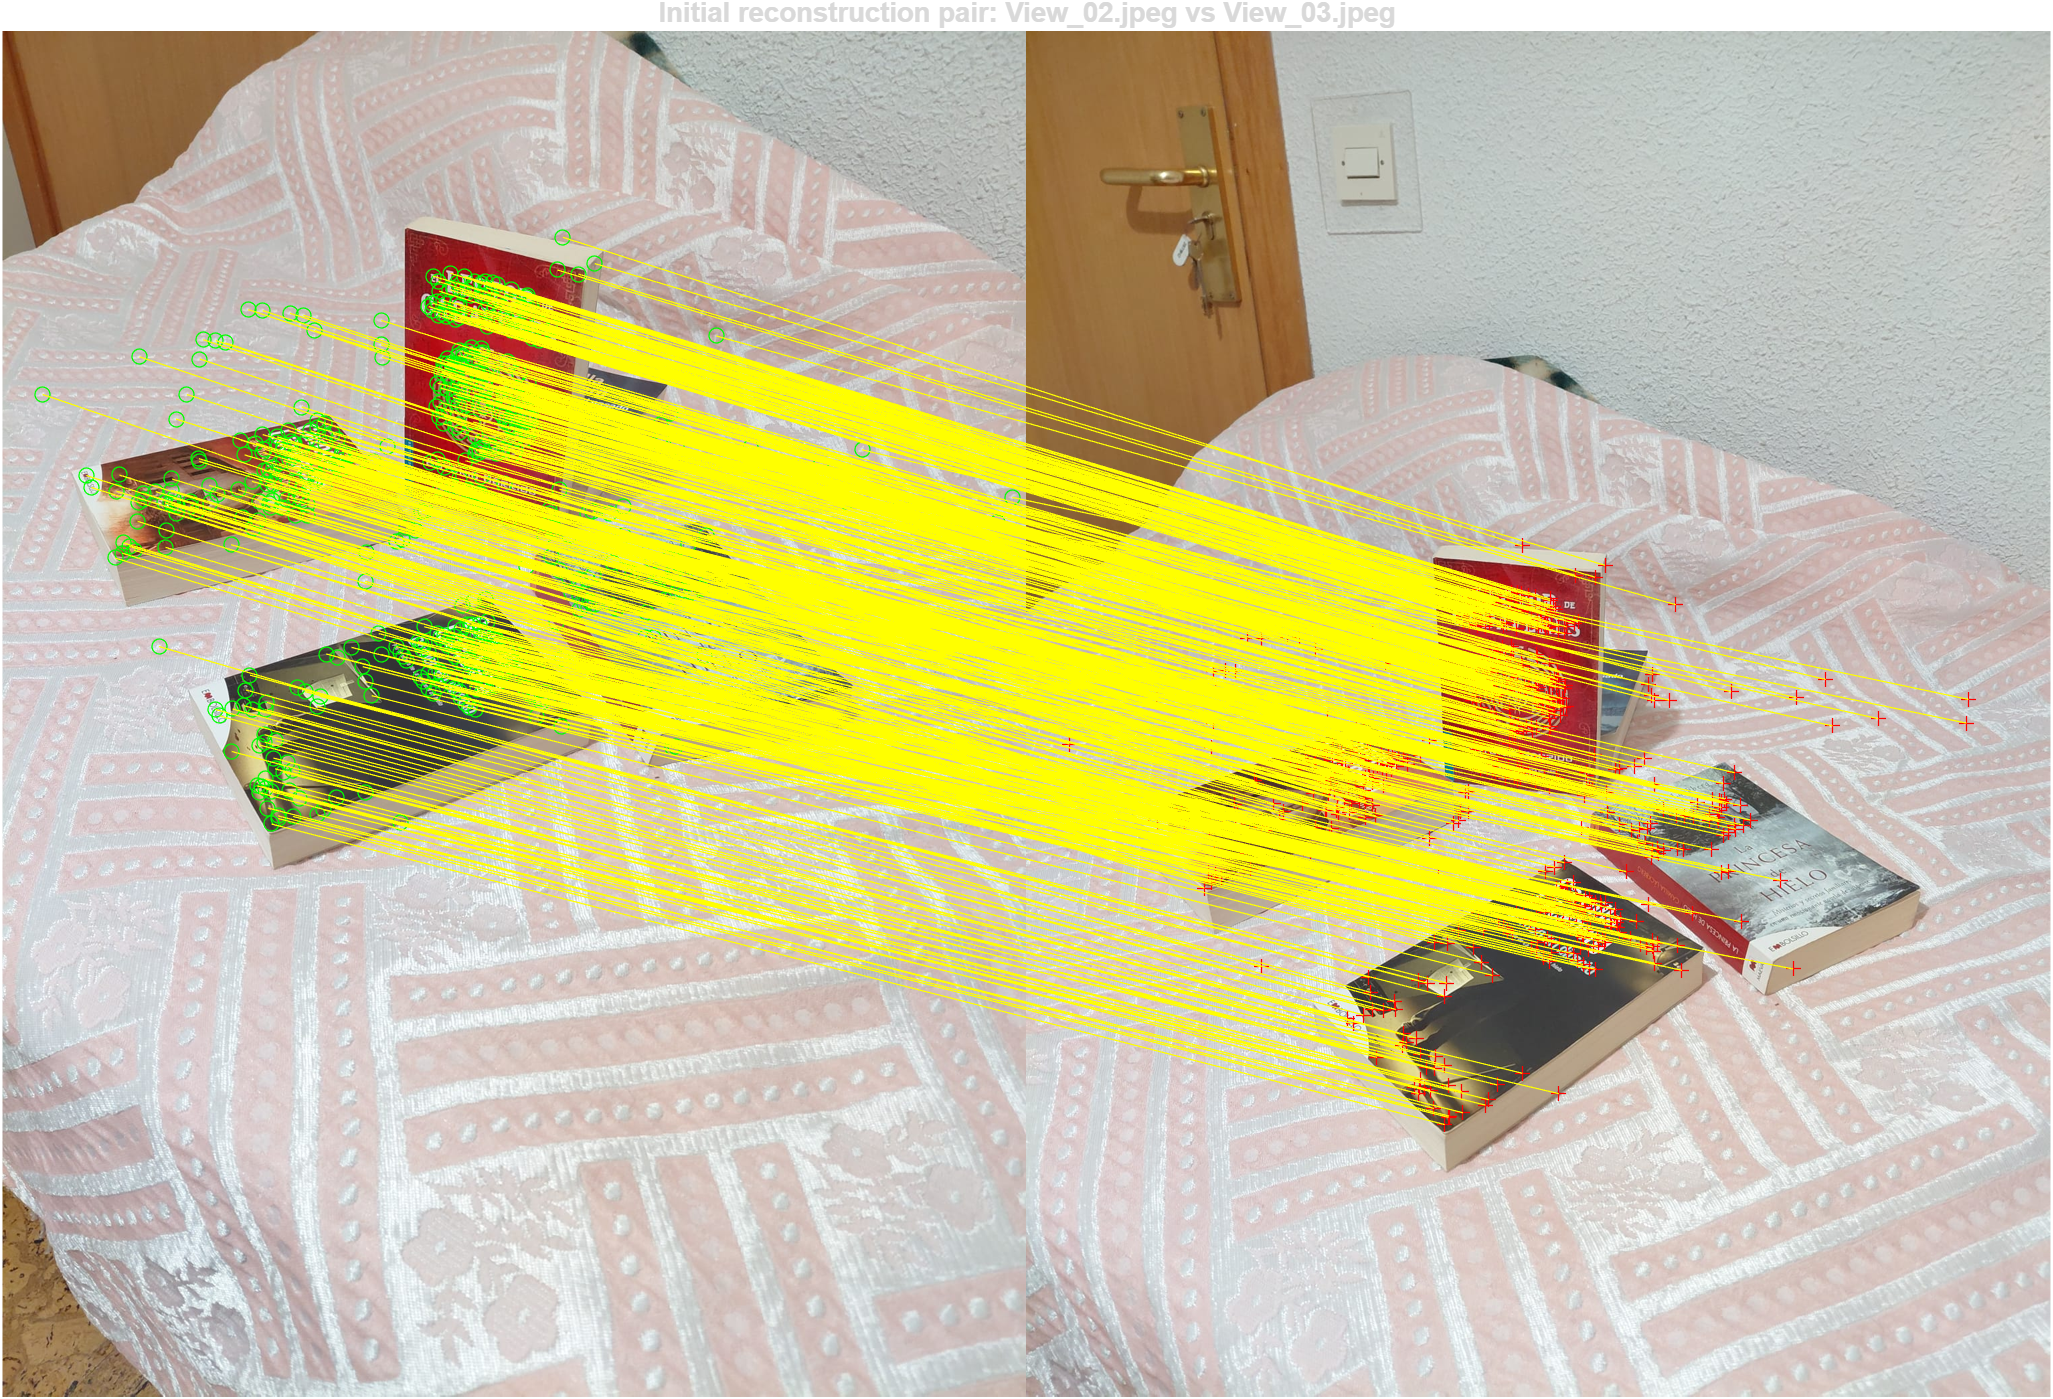
\includegraphics[width=\textwidth]{section_3/initial_pair_matches.png}
    \caption{Inlier correspondences for the initial two-camera reconstruction
             (View\_02 vs View\_03, 672 inliers, mean reprojection error
             $0.169020\,\mathrm{px}$).}
    \label{fig:sec3_initial_matches}
\end{figure}

\begin{figure}[htbp]
    \centering
    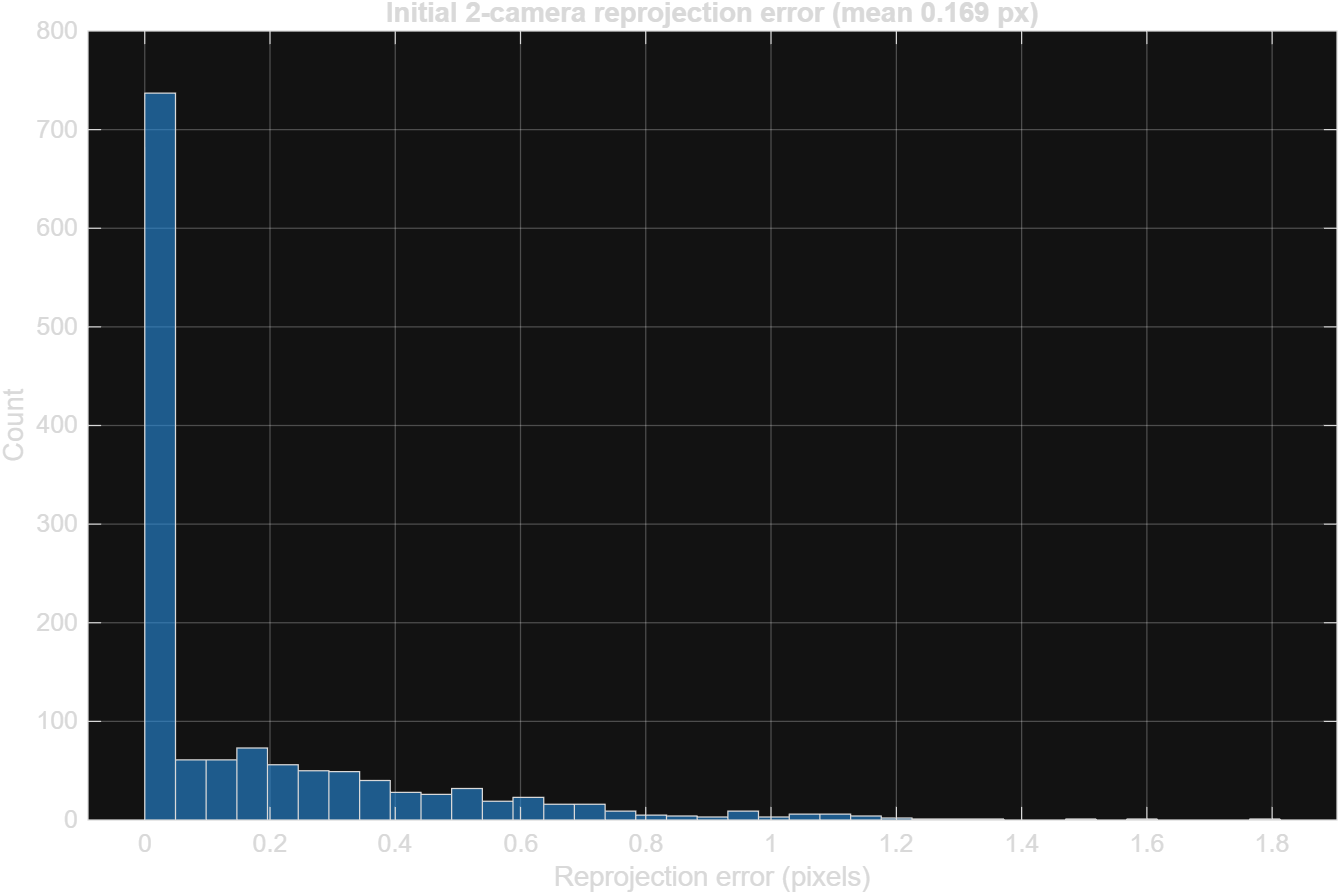
\includegraphics[width=0.70\textwidth]{section_3/initial_reprojection_hist.png}
    \caption{Reprojection error histogram after initial two-camera reconstruction
             (mean $0.169020\,\mathrm{px}$).}
    \label{fig:sec3_initial_hist}
\end{figure}

% ------------------------------------------------------------
\subsection{Resectioning and Projective Bundle Adjustment}
\label{sec:sec3_ba}
% ------------------------------------------------------------

The remaining three cameras (View\_01, View\_04, View\_05) were added sequentially
by resectioning: for each new view, the 3D-to-2D correspondences from the current
point cloud were used to estimate a new projection matrix via DLT followed by RANSAC
refinement.  After all five cameras were placed, the full projective bundle adjustment
(\texttt{BAProjectiveCalib}) was run to jointly optimise all camera matrices and
3D point positions.

\begin{table}[htbp]
\centering
\caption{Reprojection errors across the projective reconstruction pipeline.}
\label{tab:sec3_ba_errors}
\begin{tabular}{lr}
\hline
Stage & Mean reprojection error (px) \\
\hline
Initial two-camera    & 0.169020 \\
After resectioning    & 0.397073 \\
After bundle adjustment & 0.397073 \\
\hline
\end{tabular}
\end{table}

Reprojection histograms for the resectioning and bundle adjustment stages are shown
in Figures~\ref{fig:sec3_resect_hist}--\ref{fig:sec3_ba_hist}.

\begin{figure}[htbp]
    \centering
    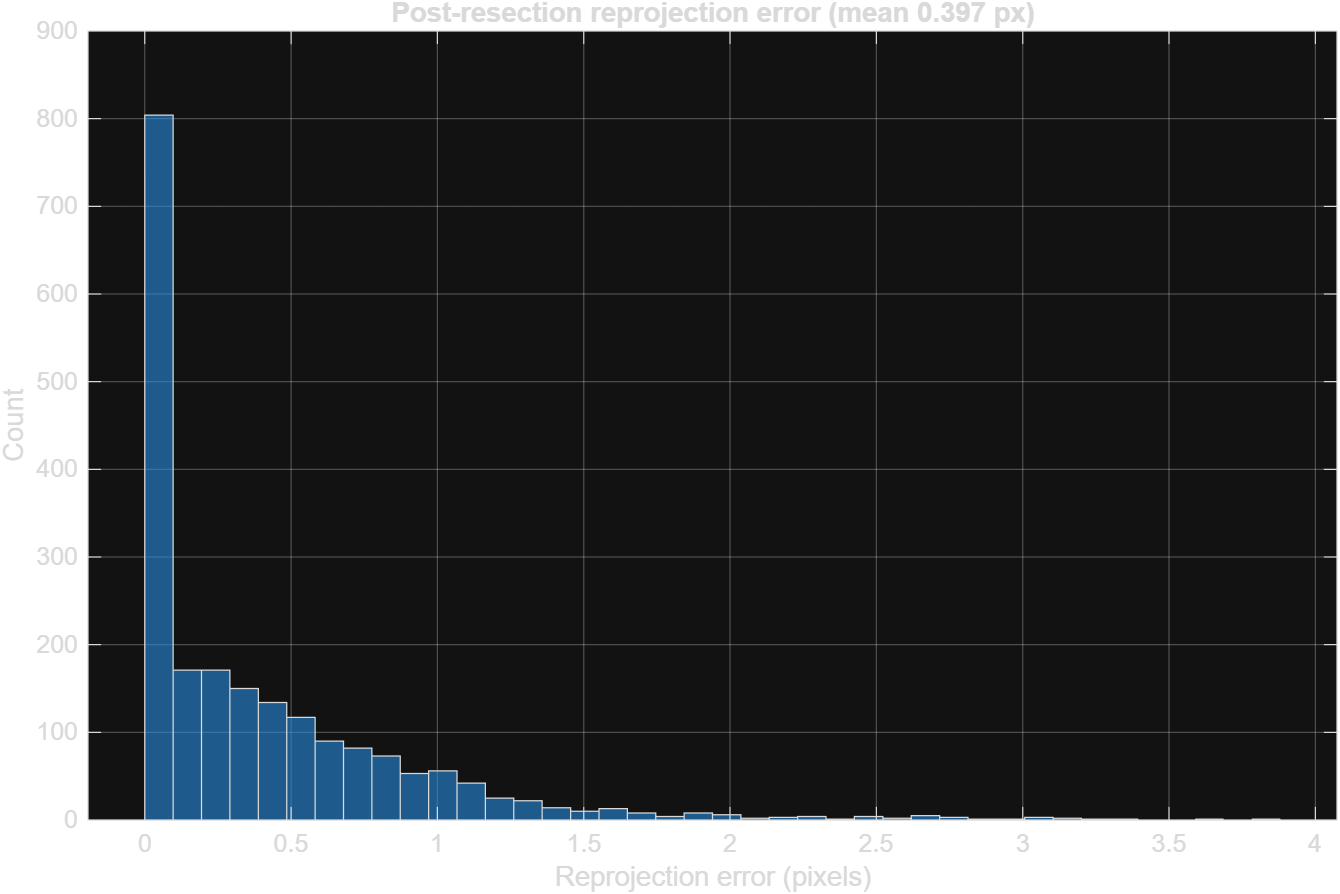
\includegraphics[width=0.70\textwidth]{section_3/resection_reprojection_hist.png}
    \caption{Reprojection error histogram after resectioning all five cameras
             (mean $0.397073\,\mathrm{px}$).}
    \label{fig:sec3_resect_hist}
\end{figure}

\begin{figure}[htbp]
    \centering
    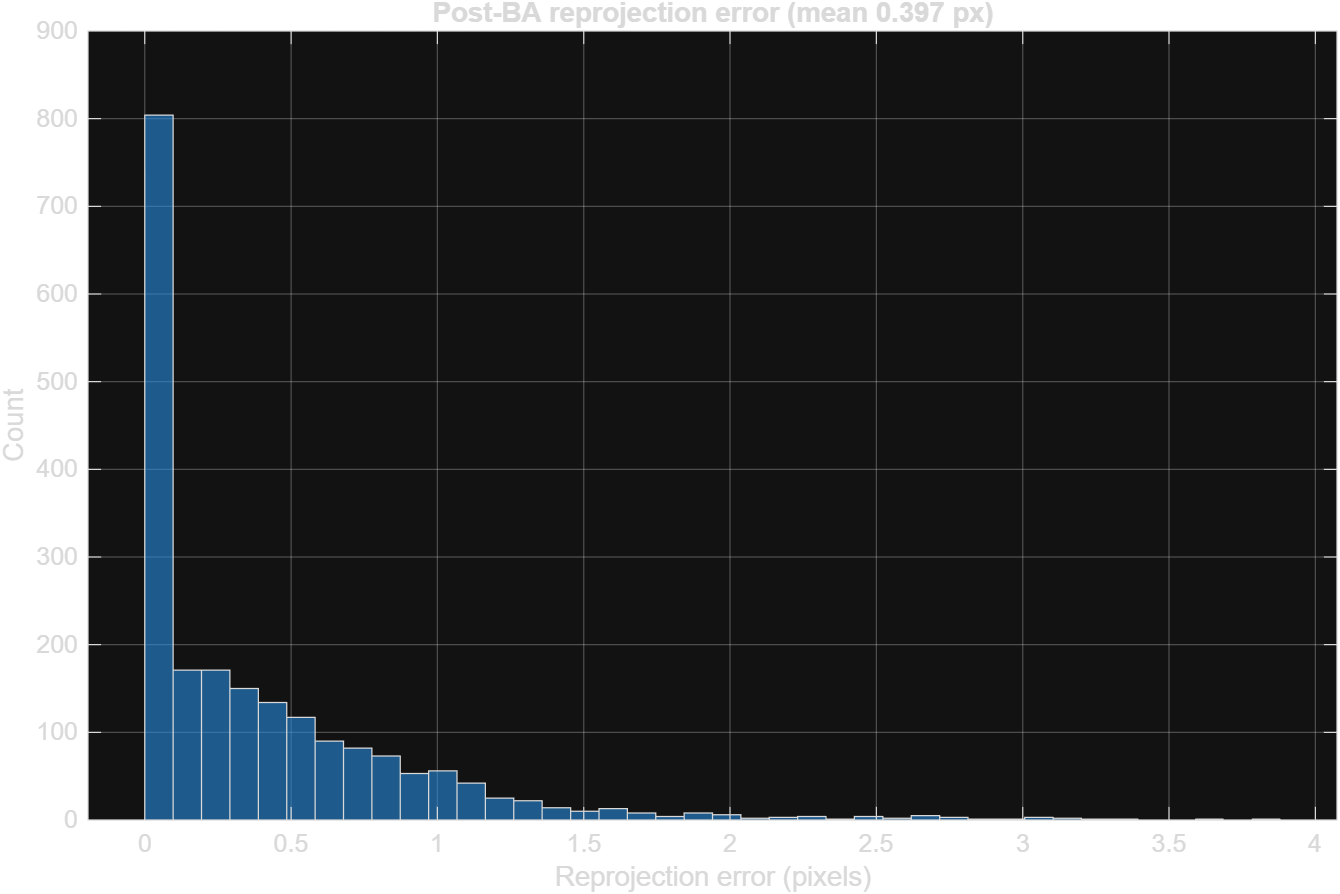
\includegraphics[width=0.70\textwidth]{section_3/ba_reprojection_hist.png}
    \caption{Reprojection error histogram after projective bundle adjustment
             (mean $0.397073\,\mathrm{px}$).}
    \label{fig:sec3_ba_hist}
\end{figure}

The slight increase from $0.169$ to $0.397\,\mathrm{px}$ after resectioning is
expected: additional cameras introduce tracks visible in fewer views with more
difficult matches.  Bundle adjustment confirmed the projective reconstruction with no
further reduction (the optimiser converged at the post-resectioning solution), which
indicates that the initial estimates were already well-conditioned.

\subsubsection*{Fundamental matrix derived from projective cameras}

As an internal consistency check, the fundamental matrix was recomputed from the
optimised projection matrices $\mathbf{P}_1$, $\mathbf{P}_2$ and compared with
$\mathbf{F}_0$.  The normalised Frobenius difference is $0.000000$, confirming that
the projective reconstruction is fully consistent with the initial epipolar geometry.
The initial matrix and the matrix recovered from the projection matrices were also
saved as \texttt{results/section\_3/initial\_F.txt} and
\texttt{results/section\_3/F\_from\_P.txt}.
The recovered matrix $\mathbf{F}_P$ (equivalent to $-\mathbf{F}_0$ up to sign) is:

\begin{equation}
\mathbf{F}_P =
\begin{bmatrix}
-0.00000003 &  0.00000001 & -0.00021335 \\
 0.00000039 & -0.00000043 &  0.00242889 \\
 0.00028406 & -0.00174221 & -0.99999547
\end{bmatrix}
\label{eq:sec3_FP}
\end{equation}

% ------------------------------------------------------------
\subsection{Essential Matrix and Euclidean Factorisation}
\label{sec:sec3_euclidean}
% ------------------------------------------------------------

The Euclidean upgrade was performed using the calibrated intrinsic matrix
$\mathbf{A}_\mathrm{sc}$ (Eq.~\eqref{eq:A_scaled}) from Section~2; this
corresponds to the direct scaled portrait calibration selected for the
processed scene images.
The Essential matrix was computed as $\mathbf{E} = \mathbf{A}_\mathrm{sc}^\top
\mathbf{F}_0\,\mathbf{A}_\mathrm{sc}$ and decomposed via SVD into four candidate
rotation-translation pairs; the correct solution was selected by the cheirality
constraint (all 3D points must lie in front of both cameras).
The scaled intrinsic matrix and Essential matrix were saved as
\path{results/section_3/euclidean_intrinsic_matrix.txt} and
\path{results/section_3/essential_matrix.txt}.

\begin{equation}
\mathbf{E} =
\begin{bmatrix}
-0.00833642 &  0.00318990 & -0.06479559 \\
 0.11904293 & -0.13917023 &  0.67991594 \\
 0.17919876 & -0.66344515 & -0.16620754
\end{bmatrix}
\label{eq:sec3_E}
\end{equation}

Candidate~10 gave $1344$ positive-depth counts and a pair-wise Euclidean
reprojection error of $6.489063\,\mathrm{px}$.
The recovered relative camera pose convention is
$\mathbf{P}_2 = \mathbf{K}[\mathbf{R}\,|\,-\mathbf{R}\mathbf{T}]$ with translation
direction:
\begin{equation}
\mathbf{t} = [0.995713,\; 0.091376,\; -0.014380]^\top
\label{eq:sec3_t}
\end{equation}

% ------------------------------------------------------------
\subsection{Final Euclidean Point Cloud}
\label{sec:sec3_cloud}
% ------------------------------------------------------------

After Euclidean factorisation all 672 tracks were triangulated in the metric frame.
The final Euclidean mean reprojection error is $4.465095\,\mathrm{px}$
(Figure~\ref{fig:sec3_euc_hist}).  This increase relative to the projective error
($0.397\,\mathrm{px}$) reflects the metric consistency constraint imposed by the
known intrinsics: the projective bundle adjustment minimises reprojection in a
projective space that has extra degrees of freedom; constraining to Euclidean space
removes those freedoms and slightly increases the algebraic reprojection cost, but
yields a metrically valid reconstruction.

\begin{figure}[htbp]
    \centering
    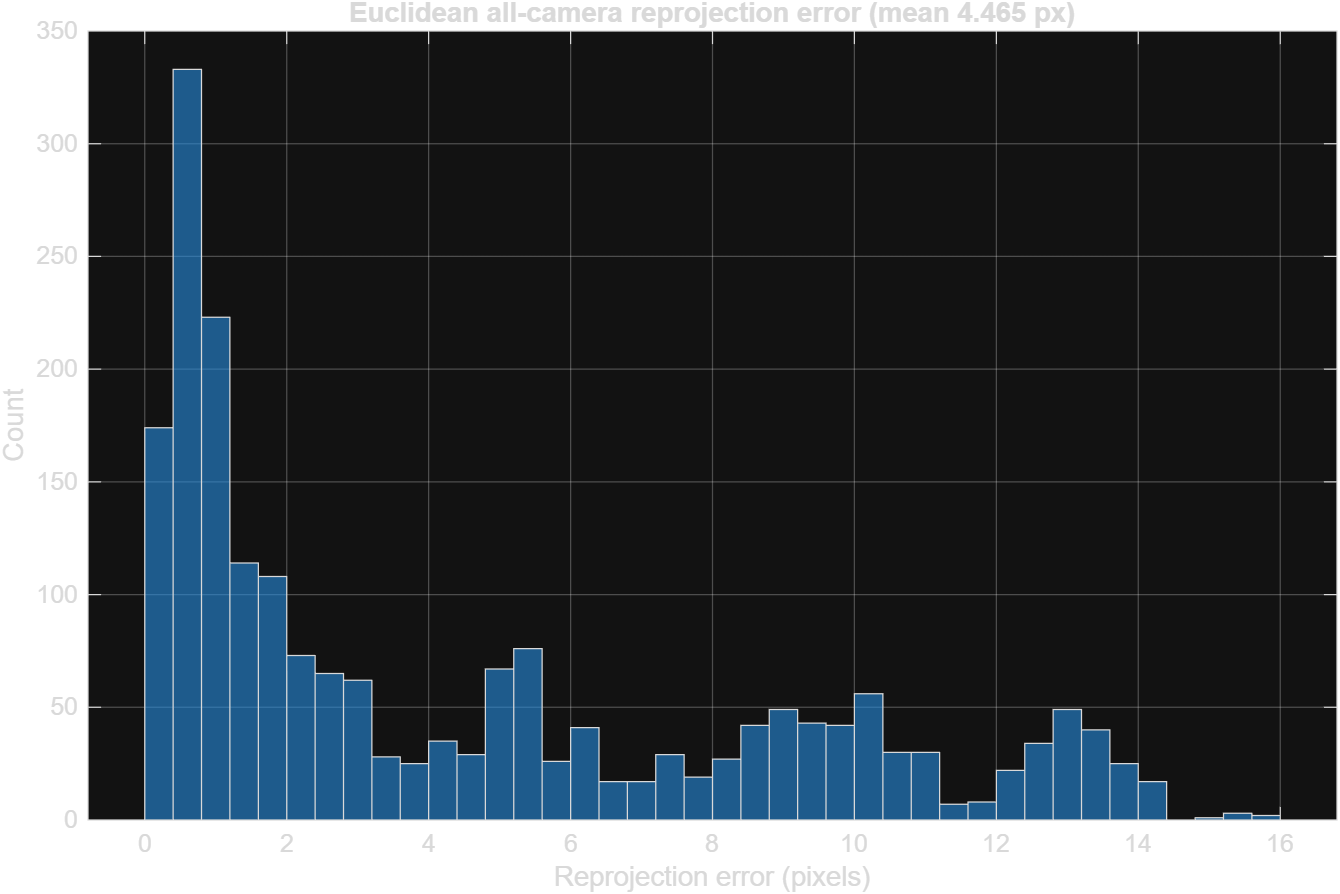
\includegraphics[width=0.70\textwidth]{section_3/euclidean_reprojection_hist.png}
    \caption{Reprojection error histogram for the final Euclidean reconstruction
             (mean $4.465095\,\mathrm{px}$).}
    \label{fig:sec3_euc_hist}
\end{figure}

Figure~\ref{fig:sec3_cloud_cam} shows the reconstructed point cloud with the estimated
camera positions from two viewpoints.
Figures~\ref{fig:sec3_scene} and~\ref{fig:sec3_colored} show the scene-only cloud and
a colour-mapped version.  The interactive MATLAB figures were saved as
\path{results/section_3/cloud_with_cameras.fig} and
\path{results/section_3/cloud_scene_only.fig}.

\begin{figure}[htbp]
    \centering
    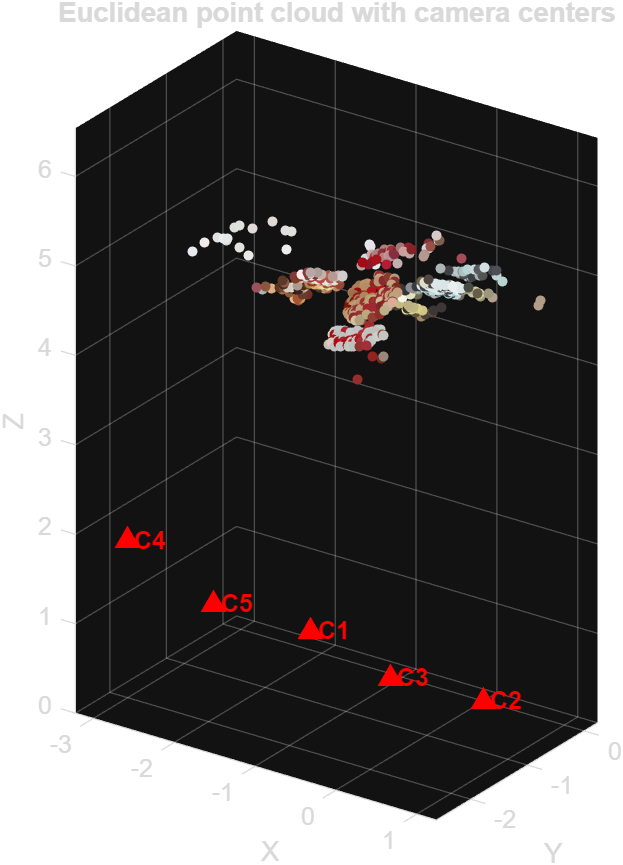
\includegraphics[width=0.48\textwidth]{section_3/cloud_with_cameras_view_1.png}
    \hfill
    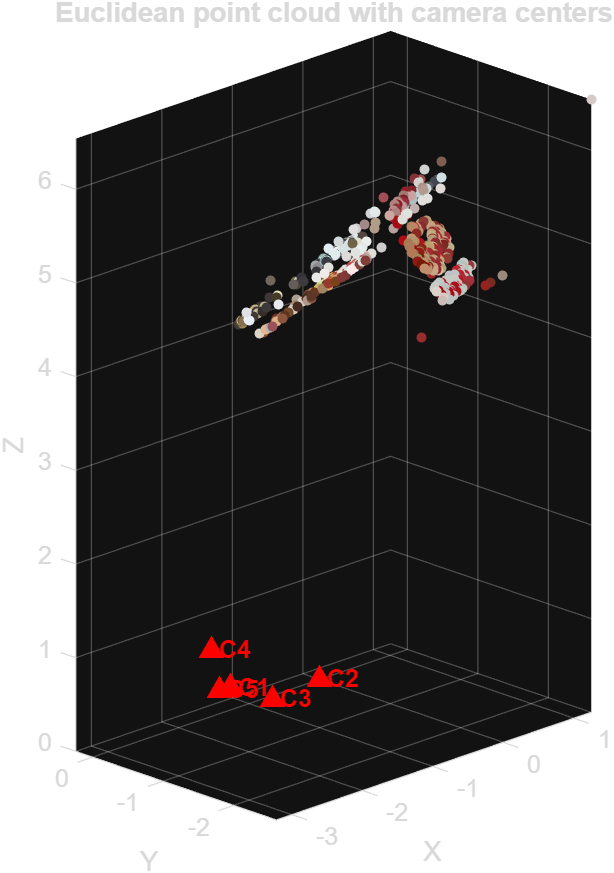
\includegraphics[width=0.48\textwidth]{section_3/cloud_with_cameras_view_2.png}
    \caption{Euclidean point cloud with estimated camera positions:
             viewpoint~1 (left) and viewpoint~2 (right).}
    \label{fig:sec3_cloud_cam}
\end{figure}

\begin{figure}[htbp]
    \centering
    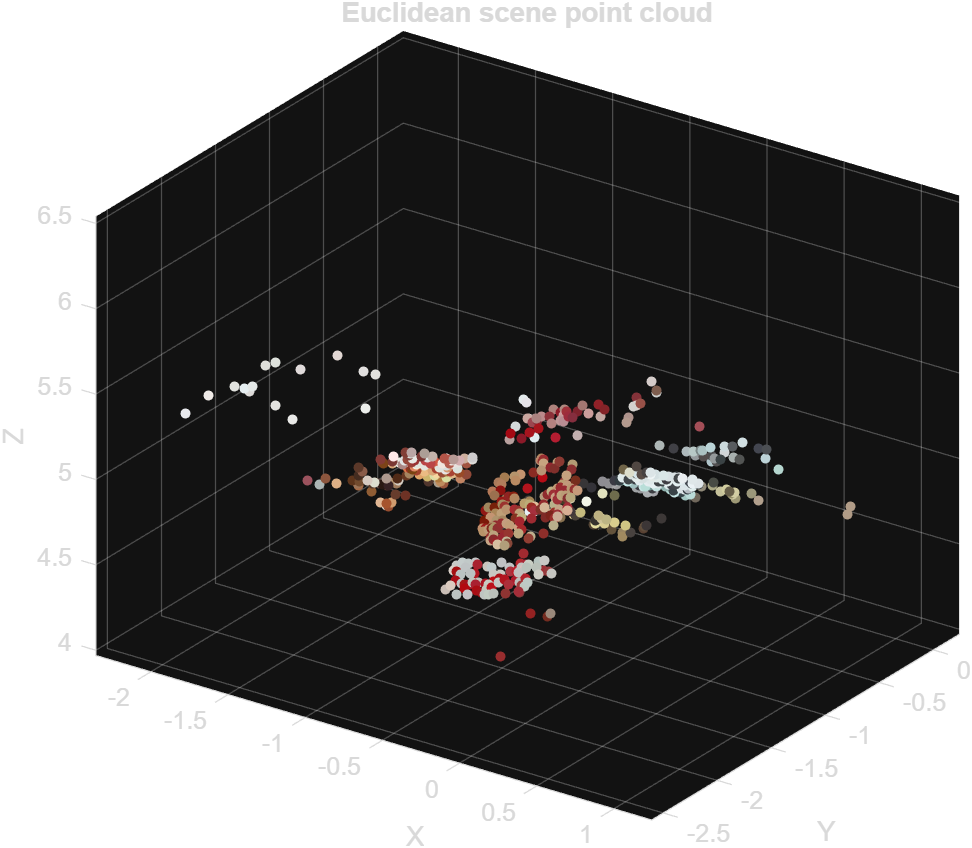
\includegraphics[width=0.48\textwidth]{section_3/cloud_scene_only_view_1.png}
    \hfill
    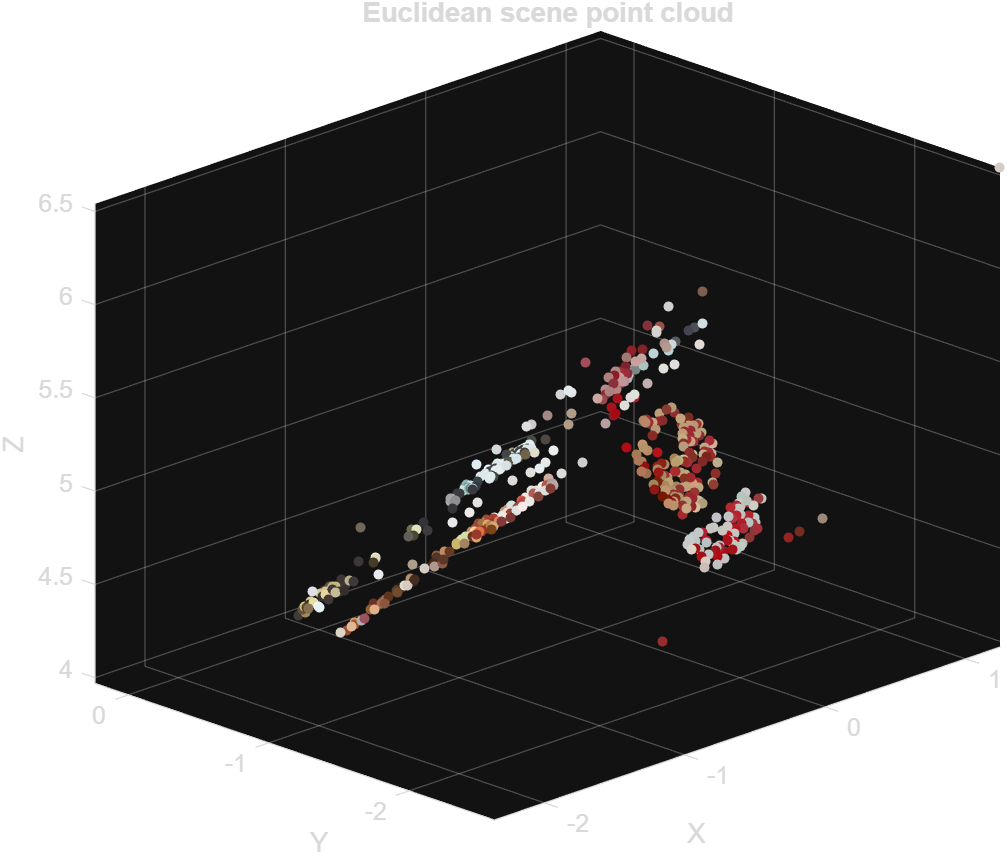
\includegraphics[width=0.48\textwidth]{section_3/cloud_scene_only_view_2.png}
    \caption{Scene-only Euclidean point cloud (cameras removed):
             viewpoint~1 (left) and viewpoint~2 (right).}
    \label{fig:sec3_scene}
\end{figure}

\begin{figure}[htbp]
    \centering
    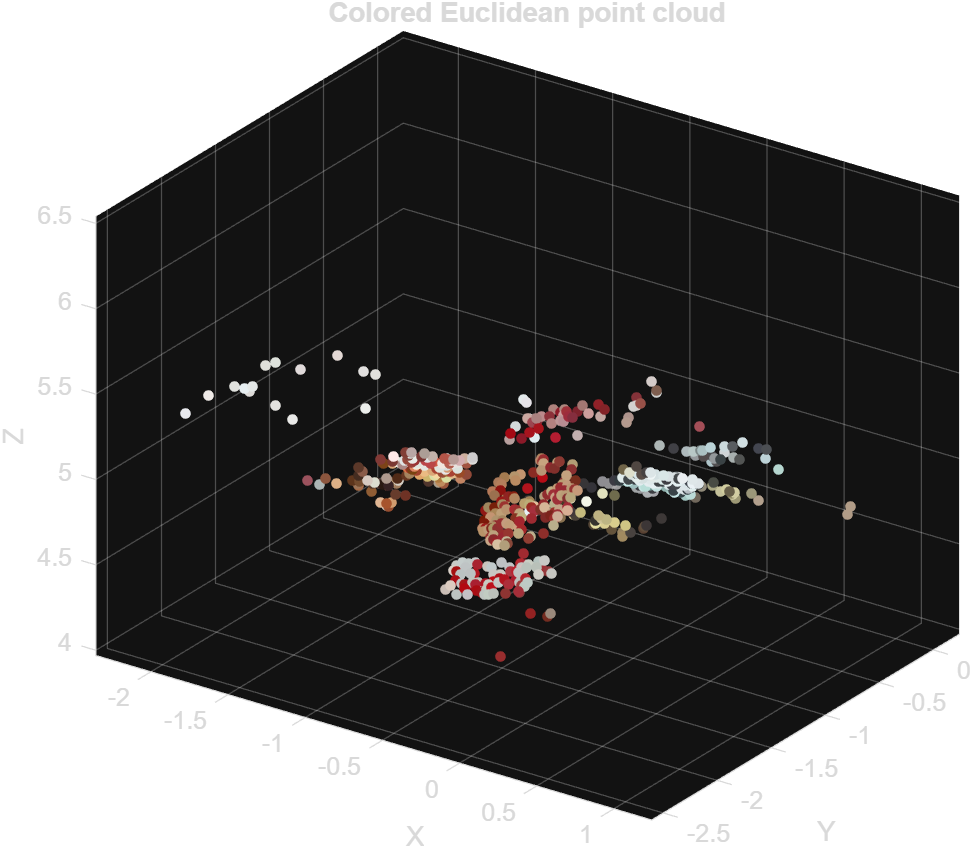
\includegraphics[width=0.80\textwidth]{section_3/colored_cloud.png}
    \caption{Colour-mapped Euclidean point cloud.}
    \label{fig:sec3_colored}
\end{figure}

\clearpage
\section{Conclusion}

This lab evaluation completed the full calibrated multi-view reconstruction workflow.
In Section~1, the screen-checkerboard calibration produced the most reliable intrinsic
matrix because it used denser and more precise point measurements than the custom
floor-tile pattern. Section~2 then used the scaled intrinsic matrix and compared several
feature-matching configurations, selecting the SIFT MATLAB strict setup on
View\_02--View\_03 because it gave the strongest fundamental-matrix support.

Section~3 used the selected feature strategy to build 672 multi-view tracks, recover an
initial projective reconstruction, add all five cameras through resectioning, and validate
the reconstruction with projective bundle adjustment. The final Euclidean upgrade
produced a metric point cloud with all five cameras valid and a mean reprojection error
of $4.465095\,\mathrm{px}$. Overall, the results are coherent with the LabFinal
requirements and demonstrate the complete transition from camera calibration to local
matching and final 3D reconstruction.

\end{document}
